\chapter{Discussion and future outlook}\label{ch:outlook}
To conclude this thesis, we shall summarise the results we have presented and raise several discussion points on the implications and extensions of our work.
This is by no means an exhaustive list; since we have provided results for a general class of stochastic differential equations, our results have the potential to be applied across a wide range of fields, well beyond the scope of this thesis.

\td{Fit in better}
Broadly speaking, our theoretical work (namely the error bound in \Cref{thm:main}) may be useful to investigate the validity of SDE linearisations in application domains such as Stochastic Parameterisation \citep{BernerEtAl_2017_StochasticParameterizationNew,Palmer_2019_StochasticWeatherClimate,LeutbecherEtAl_2017_StochasticRepresentationsModel} or Data Assimilation \citep{BudhirajaEtAl_2019_AssimilatingDataModels,ReichCotter_2015_ProbabilisticForecastingBayesian,LawEtAl_2015_DataAssimilationMathematical}, or to improve such linearisations by monitoring the skew or kurtosis.

The later sections of this chapter cover:
\begin{itemize}
	\item In \Cref{sec:disc_sigma}, we discuss approaches to selecting the diffusivity matrix \(\sigma\).
	\item In \Cref{sec:disc_bc}, we discuss the difficulties that boundary conditions can present to both the formulation of an SDE and our methods.
	\item In \Cref{sec:disc_fp}, we introduce the Fokker-Planck equation, which provides an alternative view of the solution of a stochastic differential equation, and discuss how this perspective can further our theoretical understanding.
	\item In \Cref{sec:disc_levy}, we discuss the possibility of replacing the Wiener process in the driving stochastic differential equation with a more general L\'evy process.
	\item In \Cref{sec:disc_higher}, we discuss the extension of our theory in \Cref{ch:linear_theory} to include higher-order terms in the small-noise expansion of the SDE.
	\item In \Cref{sec:s2_disc}, we discuss the implications of our extension to stochastic sensitivity and the applications thereof.
	\item In \Cref{sec:epi_disc}, we draw analogies between our theoretical work and results for the limits of population processes, a class of stochastic models evolving on a discrete state space.
	      This suggests that our tools can be applied to a broader class of stochastic models.
	      The section culminates in a 5-dimensional implementation of the Gaussian computation outlined in \Cref{ch:linear_numerics} on a data-informed model for the spread of Ebola.
\end{itemize}

We began the main contribution of this thesis in \Cref{ch:linear_theory}, where we provided and justified a framework for computing linearisations of stochastic differential equations.
We provided in \Cref{thm:main} an explicit bound on the error between the solution of a small-noise nonlinear stochastic differential equation and an easily computable linearisation approximation, building upon previous studies \citep{Blagoveshchenskii_1962_DiffusionProcessesDepending,FreidlinWentzell_1998_RandomPerturbationsDynamical,Sanz-AlonsoStuart_2017_GaussianApproximationsSmall}.
The linearisation approximation is used across many applications and contexts \citep[e.g.]{Jazwinski_2014_StochasticProcessesFiltering, Sanz-AlonsoStuart_2017_GaussianApproximationsSmall,KaszasHaller_2020_UniversalUpperEstimate,ArchambeauEtAl_2007_GaussianProcessApproximations}, but often without a clear mathematical justification.
The theory applies to fully non-autonomous SDEs with multiplicative noise and a random initial condition.
Our bound is written in terms of a scaling of the diffusivity matrix and a measure of the uncertainty in the initial condition using the \(L_r\)-norm.
A comparison in \Cref{sec:comparison} suggests that our bound on the moments is tighter than implied by the gold standard in the literature (a comparable bound on the Kullback-Leibler divergence by \citet{Sanz-AlonsoStuart_2017_GaussianApproximationsSmall}).
% Unlike the bounds in other literature \citep[e.g.]{Blagoveshchenskii_1962_DiffusionProcessesDepending,FreidlinWentzell_1998_RandomPerturbationsDynamical}, by explicitly identifying the dependence of our bound on when the noise in the SDE is multiplicative and the drift nonlinear, we were also able to highlight two application-relevant special cases: when the initial condition is fixed, and when it is Gaussian.
We also provided in \Cref{thm:limit_sol} and \Cref{cor:limit_moments} an explicit characterisation of the distribution of the solution to the linearised SDE, enabling efficient approximation of the original nonlinear SDE using solutions to the corresponding deterministic equation, whereas previously special cases of these computations were dispersed across other literature \citep[e.g.]{Jazwinski_2014_StochasticProcessesFiltering,Sanz-AlonsoStuart_2017_GaussianApproximationsSmall,SarkkaSolin_2019_AppliedStochasticDifferential}.
In \Cref{sec:theory_fixed} and \Cref{sec:theory_gauss} we highlighted two application-relevant special cases: when the initial condition is fixed and when it is Gaussian, respectively.
Coupled with the efficient \citet{Mazzoni_2008_ComputationalAspectsContinuous} method (summarised in \Cref{sec:mazzoni}) to compute the moments of the linearisation solution, we have provided a rigorous and practical framework for approximating small-noise SDEs with linearisations about the solutions of their corresponding deterministic systems.

Our next contribution was to extend the stochastic sensitivity tools introduced by \citet{Balasuriya_2020_StochasticSensitivityComputable}.
Stochastic sensitivity was hitherto derived as the variance of an unknown limiting distribution and could only be computed in two spatial dimensions.
We provided a new definition of stochastic sensitivity that extends the original to any number of dimensions and is computable as the operator norm of the covariance matrix of the linearised SDE (for which we outlined the computation in \Cref{thm:limit_sol} and \Cref{cor:limit_moments}).
We have also established that the limiting distribution in question is Gaussian, as the computation is related directly to a linearised SDE with a fixed initial condition.
This may provide insight into properties of stochastic sensitivity as a means of uncertainty quantification in \emph{any} model (not just in the fluids context) where an \(n\)-dimensional state variable evolves according to a ``best available'' deterministic model.

With three example SDEs in 1- and 2-dimensions in \Cref{ch:linear_numerics}, we validated the form of our theoretical error bound and showed heuristically that the solutions approach that of their respective linearisations in the limit of small noise.
In particular, we found that the strong error scales with the initial uncertainty and ongoing uncertainty exactly as predicted.
% Thus, we have provided a rigorous (in the sense of a bound and a limit) justification for using such approximations when the noise in the model is small, and a framework for rapid computation of the first two moments of the linearisation.
We also demonstrated the new computation of stochastic sensitivity in two dimensions (in \Cref{sec:compute_s2_2d}) and, for the first time, in 3-dimensions (in \Cref{sec:comput_s2_3d}).

Although linearisation approximations of SDEs have proven to be useful in both applications and as a theoretical tool (e.g.\ stochastic sensitivity), in \Cref{ch:gmm} we highlighted that the limitations of using such approximations, particularly when the linearisation solution is a Gaussian process.
A Gaussian approximation cannot capture features such as skew and multimodality, despite these distinctly non-Gaussian attributes arising both in the solutions of nonlinear and multiplicative noise SDEs and observed statistics \citep{SuraEtAl_2005_MultiplicativeNoiseNonGaussianity,del-Castillo-Negrete_1998_AsymmetricTransportNonGaussian,BraccoEtAl_2000_VelocityProbabilityDensity}.
To overcome these limitations while still taking advantage of the computationally efficient linearisation approximation, we proposed an \emph{ad hoc} algorithm that uses a splitting process to approximate SDE solutions with a Gaussian mixture model.
Each component of the mixture model arises from a solution of the SDE linearised about a \emph{different} deterministic trajectory, which can capture uncertainty in different regions of the state space.
With a simple propagation-splitting procedure, the algorithm can capture multimodality, skewness, and other departures from Gaussianity to improve upon a single Gaussian component.
Another advantage of this algorithm is that it provides an analytically available probability density function, as opposed to stochastic samples, which require an additional step to estimate the density function.
Our aim throughout was to outline the algorithm and demonstrate its potential on several simple implementations, rather than explore the specifics of each step or perform a mathematical analysis.
Instead, we briefly discussed some suggestions for these specifics throughout \Cref{ch:gmm} while leaving a thorough investigation further as future work.

In \Cref{ch:appls}, we applied the developments of the previous chapters to a data-driven model.
Using satellite-measured velocity data, we constructed two 2-dimensional models for the motion of a drifter on the surface of the Gulf Stream in the North Atlantic Ocean.
The first was a purely deterministic ordinary differential equation, using only the interpolated velocity data.
The second was a stochastic differential equation that `improved' upon the ODE by accounting for measurement errors in the velocity data and unresolved effects due to the spatial resolution of the data.
By computing stochastic sensitivity, we used the stochastic model to diagnose the reliability of the deterministic model over the spatial domain of the data.
We then focussed our attention on a single solution trajectory, corresponding to the motion of the drifter starting from a fixed initial condition.
The stochastic model produced a highly non-Gaussian distribution (estimated from Euler-Maruyama samples) for the position of the drifter at a later time.
We compared to this empirical distribution the Gaussian approximation arising from a linearisation of the stochastic model about the deterministic trajectory but found that the Gaussian density was limited in representing the key features of this distribution.
Motivated by this, we explored two simple implementations of the mixture model algorithm, using the Hellinger distance to `tune' the splitting times with reference to the stochastic samples.
The mixture model showed highly promising results on this example trajectory; with only 2 splits and 25 components, the algorithm could closely recreate the highly non-Gaussian distribution (in \Cref{fig:na_2split_best}).



\section{Selecting the diffusivity matrix}\label{sec:disc_sigma}
A powerful advantage of our framework is that the diffusivity matrix \(\sigma\) may vary spatiotemporally, allowing for multiplicative noise.
Multiplicative noise is often ignored in practice, because of difficulties in analytic work \citep{SanchoEtAl_1982_AnalyticalNumericalStudies} and generating numerical realisations efficiently \citep{MoraEtAl_2017_StableNumericalScheme}.
Despite these challenges, multiplicative noise is often necessary in practice \citep[e.g.]{Sura_2003_StochasticAnalysisSouthern,KamenkovichEtAl_2015_PropertiesOriginsAnisotropic}.
% For example, \citet{SuraEtAl_2005_MultiplicativeNoiseNonGaussianity} showed that multiplicative noise on linear dynamics can model departures from Gaussianity observed in climate statistics, as opposed to nonlinear dynamics with only additive noise.
Such noise can also arise from experimental and observational considerations that are otherwise ignored in the deterministic model, such as cloud cover when using satellite measurements or nonuniformity across the field of view of a camera.
This raises the question of exactly \emph{how} to specify \(\sigma\), particularly when the aim is to measure uncertainty in a model that is only initially specified deterministically.
If there is no \emph{a priori} knowledge about the spatiotemporal structure of the noise, then the default choice of \(\sigma = I\) addresses a generic situation in which noise is uniformly ascribed to each component of the state.
In \Cref{ch:appls}, we took a na\"ive approach to include measurement error estimates in our model by selecting \(\sigma\) so that \(\sigma\sigma^{\T}\) corresponded to a variance.
However, there is potential for a more informed construction of \(\sigma\) that accounts for the many limitations of the deterministic model.
For instance, the velocity field in the deterministic ODE was constructed by interpolating the observed data, which was only available on a finite spatiotemporal grid.
One could encode in \(\sigma\) the error introduced by using this interpolant, for example, reducing the magnitude of the diffusivity at gridpoints and increasing it further away.
The impact of interpolation, quantified by a multiplicative noise SDE, warrants a full investigation, in which stochastic sensitivity could provide a computable quantification of the impact of this introduced uncertainty \citep{FangEtAl_2020_DisentanglingResolutionPrecision,FangOuellette_2021_AssessingInformationContent}.
It is also pertinent to note that the driving Wiener process in the SDE model need not have the same dimension as the state variable.
The model can thus account for different sources of uncertainty that do not need to be attributed directly to the components of the velocity field.
This was an implicit limitation of the original stochastic sensitivity work \citep{Balasuriya_2020_StochasticSensitivityComputable}, where the Wiener process could only be 1- or 2-dimensional.
For instance, in a model containing several unknown or estimated parameters, we could encode the uncertainty in these parameters with the components of a Wiener process.
This would lead to a certain construction of \(\sigma\) from the relationship between those parameters and the vector field of the ODE model---we provided a simple example of this in our 2-dimensional toy model in \Cref{ch:linear_numerics}, where we devised a spatially varying diffusion matrix \cref{eqn:jet_ex_sigma} by attributing the uncertainty to two of the model parameters.

There are many application-specific methods available for estimating \(\sigma\) directly from observed data, e.g.\ via statistical estimation \citep{CotterPavliotis_2009_EstimatingEddyDiffusivities} or the Bayesian inference approach of \citet{YingEtAl_2019_BayesianInferenceOcean} in the context of ocean modelling.
For a review of the statistical estimation of the diffusion matrix from noisy data, see \citet{NielsenEtAl_2000_ParameterEstimationStochastic}.
Coupling these approaches with our methods could provide a complete and practical framework for characterising uncertainty using only observed trajectory data, without the need to specify directly the diffusion matrix as part of the model.
In oceanography, a common approach is to specify the diffusion term as part of a physics-informed model \citep{BerloffMcWilliams_2002_MaterialTransportOceanic}.
For example \citep{vanSebilleEtAl_2018_LagrangianOceanAnalysis,LiEtAl_2023_StochasticDataDrivenParameterization}, in modelling Lagrangian particles, the movement of material via unresolved subgrid processes is quantified as diffusive transport.
This then leads to the specification of an advection-diffusion equation with a spatially varying diffusivity that specifies the time-evolution of the spatial distribution of Lagrangian particles.
Via the Fokker-Planck equation (to be introduced in \Cref{sec:disc_fp}), this purely deterministic formulation is equivalent to a stochastic differential equation with a drift and diffusion matrix relating to the terms of the advection-diffusion equation.
A similar approach is employed in stochastic parameterisations of atmospheric convection \citep{WilsonSawford_1996_ReviewLagrangianStochastic}.
We must emphasise, however, that the specification of the diffusion term is an open question and depends on the specifics of the situation and modelling choices.
Our theory is general enough to cover all of these aforementioned cases.

\section{Boundary conditions}\label{sec:disc_bc}
In many practical situations, we can enforce boundary conditions on the evolution of our state variable.
These conditions are typically informed by physical aspects of the model, such as expecting that a variable of interest is non-negative, the presence of impermeable boundaries, or limitations of the underlying data.
The Gulf Stream example in \Cref{ch:appls} provided one such situation.
Firstly, the subset of altimetry data that we used was only available on a finite spatial region, which is almost always the case in data-driven models.
Outside of this region, we have no data and so there is an implicit boundary: once a trajectory leaves the data domain we can no longer propagate it forward or make further inferences.
We also expected, from physical considerations, that drifter trajectories cannot move onto the regions of land within the dataset, creating impermeable boundaries.
For an ordinary differential equation, boundary conditions usually do not pose a significant problem.
However, the treatment of these boundaries in stochastic differential equations can be more complicated, requiring adjustments to both the drift and diffusion.
There are two primary types of boundary conditions: absorbing, which acts as a set of fixed points, and reflecting, where the trajectories are `pushed away' from the boundary.
Reflecting boundary conditions can be enforced with a modification of the drift---see \citet{Pilipenko_2014_IntroductionStochasticDifferential} for an introduction.
An absorbing boundary condition presents a more difficult proposition, such as requiring specialised numerical schemes \citep{Mannella_1999_AbsorbingBoundariesOptimal}, causing a breakdown in the Markovian behaviour of the solution \citep{Munoz_1998_NatureDifferentTypes}, and even causing ambiguity in the interpretation of the driving noise \citep{CorrealesEscudero_2019_ItoVsStratonovich}.

% can be accounted for by setting both the drift and diffusivity in the stochastic differential equation to zero on the boundary \citehere.
% However, such adjustments will often violate the requirements of smoothness in these terms set out in \Cref{hyp:smooth}.
% Regardless, these SDEs are well-defined and can be proven to have solutions under relaxed continuity conditions.\lb{Need to double check all this}

Even without considering these technical modifications, there are difficulties in using our tools in the presence of boundaries.
An \(n\)-dimensional Gaussian density has support on the entirety of \(\R^n\), meaning that for any sensible non-empty region in \(\R^n\), there is a non-zero probability that a random variable following a non-degenerate Gaussian distribution takes a value in that region.
This property means that a Gaussian approximation, such as that arising from the linearisation, cannot capture boundary behaviour.
Our Gaussian mixture model consequently suffers from the same limitation.
A further difficulty in the mixture model algorithm is the selection of new components when splitting; without adjustment, the new components may be placed across boundaries and violate conditions on the state.
This can be avoided by appropriately adjusting the new components and their weights, for instance, but is another practical issue that needs further consideration.
We avoided complications in our Gulf Stream example by ensuring that the target densities and the evolution of solution trajectories were sufficiently far from the boundaries.
The probability that a solution or the resulting approximations were close to the boundaries was then negligible.
Without these considerations, however, the boundaries pose a significant problem---any inferences that use the SDE linearisation, notably stochastic sensitivity, cannot be trusted near those boundaries.
When generating realisations, a na\"ive approach to handling these boundaries is to discard any trajectories that leave the spatial domain.
In a similar vein, one may adjust the approximate probability density functions obtained by our techniques by discarding probability mass that violates the boundary conditions and renormalising the function.
This approach is not supported with a mathematical justification, however, and would not account for the behaviour of the solution at the boundary (e.g.\ absorbing versus reflecting).
A more intriguing prospect is to adjust the linearised SDEs themselves to include these boundary conditions and attempt to find an appropriate solution.
This is not easy, however, due to the aforementioned theoretical modifications that must be made to the formulation and solution approach to a stochastic differential equation in the presence of boundaries.
Any headway in this direction could overcome one of the most significant limitations of Gaussian/linearisation approximations of stochastic differential equations.


% \section{Further theoretical developments}
% In this section, we briefly postulate three extensions to the theoretical results presented in \Cref{ch:linear_theory}.

\section{The Fokker-Planck equation}\label{sec:disc_fp}
The Fokker-Planck equation is a partial differential equation that describes the time evolution of the probability density function of the solution to a stochastic differential equation.
Given an SDE
\begin{equation}
	\dif x_t = u\!\left(x_t,t\right)\dif t + \sigma\!\left(x_t,t\right)\dif W_t,
	\label{eqn:fp_sde}
\end{equation}
the probability density function \(\rho\) for the solution to \cref{eqn:fp_sde} at time \(t\) solves the corresponding Fokker-Planck (FP) equation \citep{Risken_2012_FokkerPlanckEquationMethods}
\begin{equation}
	\dpd{\rho\!\left(x,t\right)}{t} = \frac12\nabla\cdot\nabla\cdot\left(\rho\!\left(x,t\right)\sigma\!\left(x,t\right)\sigma\!\left(x,t\right)^{\T}\right) - \nabla\cdot\left(\rho\!\left(x,t\right) u\!\left(x,t\right)\right)
	\label{eqn:fp_eqn}
\end{equation}
subject to some initial density \(\rho\!\left(x,0\right)\) given by the distribution of the initial condition to \cref{eqn:fp_sde}.
% For a fixed and deterministic initial condition \(y_0 = x\), the corresponding initial condition to \cref{eqn:fp_eqn} is the Dirac-delta distribution centred at \(x\).
% To ensure that the solution is a valid probability density function on \(\R^n\), for any \(t \in [0,T]\), \(\rho\) must satisfy
% \begin{subequations}\label{eqn:fp_valid_pdf}
% 	\begin{align}
% 		\int_{\R^n}{\rho\left(x, t\right)\dif x} = 1, \label{eqn:fp_valid_pdf_norm} \\
% 		\lim_{x \to \infty}\rho\left(x,t\right) = 0. \label{eqn:fp_valid_pdf_limit}
% 	\end{align}
% \end{subequations}
Solving the Fokker-Planck equation provides an alternative method for finding the solution to a stochastic differential equation; rather than working directly with the stochastic trajectories that solve \cref{eqn:fp_sde}, we instead seek solutions to a partial differential equation.
Our work could both contribute to understanding the Fokker-Planck equation and conversely, make use of this alternative view on SDEs.
We could extend our theoretical work on SDE linearisations to consider the corresponding Fokker-Planck equations.
We presented the solution to the linearised SDE in \Cref{thm:limit_sol}, for which we can derive an expression for the probability density function---the PDF is a Gaussian density or can otherwise be computed as the convolution between a Gaussian and the initial condition PDF.
Therefore, we have solutions available to the Fokker-Planck equation corresponding to the linearised SDE.
% The linearised stochastic differential equation has a corresponding Fokker-Planck equation, for which the solution is available---the probability density function of the linearisation solution, which is Gaussian for a fixed initial condition or can otherwise be computed as a convolution between a Gaussian and the initial condition PDF, is the solution to the corresponding Fokker-Planck equation.
If we could understand the relationship between the Fokker-Planck equations of the original SDE and the linearisation, this would accordingly offer insight into the relationship between the probability density functions of the respective SDE solutions.
Such understanding cannot be inferred from our bound on the expectation in \Cref{thm:main} alone.

Secondly, the Fokker-Planck equation cannot be solved analytically except for simple cases and so is typically approximated.
There are two approaches to numerically solving the Fokker-Planck equation: either by generating many stochastic realisations by solving the corresponding SDE \cref{eqn:gen_sde} numerically and using a density estimation method \citep{Silverman_2017_DensityEstimationStatistics}, or by directly solving the Fokker-Planck equation with a finite-difference or finite-element scheme \citep{PichlerEtAl_2013_NumericalSolutionFokker}.
Both approaches have practical difficulties, including poor scaling with dimensionality and the enforcement of boundary conditions.
% \begin{itemize}
% 	\item \textbf{Dimensionality:} In high-dimensional systems, solving the Fokker-Planck equation numerically is computationally prohibitive, requiring either  a large number of stochastic samples or a fine spatial discretisation to be accurate.
% 	\item \textbf{Boundary conditions:} The Fokker-Planck equation is often defined on an unbounded domain with the zero-limit constraint \(\lim_{\norm{x} \to \infty}\rho\!\left(x,t\right) = 0\), which presents additional computational difficulties.
% 	\item \textbf{Normality constraints:} The Fokker-Planck equation must be solved with additional normality condition---the solution represents a probability density function, and so must always be bounded and integrate to 1---which enforces an additional constraint on any numerical solution.
% \end{itemize}
These difficulties mean that the computational cost of solving the Fokker-Planck equation is considered impractical in \(3\)- or higher dimensions \citep{ZhaiEtAl_2022_DeepLearningMethod,Li_2019_DatadrivenMethodSteady,AllawalaMarston_2016_StatisticsStochasticallyForced,AndersonFarazmand_2024_FisherInformationShapemorphing}.
% There has been much recent interest in developing data-driven methods for solving the Fokker-Planck equation directly \citep{ZhaiEtAl_2022_DeepLearningMethod,Li_2019_DatadrivenMethodSteady,AllawalaMarston_2016_StatisticsStochasticallyForced,AndersonFarazmand_2024_FisherInformationShapemorphing}.
The linearisation approximation and our Gaussian mixture model algorithm both provide analytic probability density functions and are both efficient methods that scale reasonably with dimension.
These methods may therefore be viewed as approximate solution methods to the Fokker-Planck equation that overcome the computational limitations of numerical solutions.
Understanding the relationship between SDE linearisations and the Fokker-Planck equation may provide an avenue for further developing the mixture model algorithm.
The aim of the mixture model is to approximate the probability density function of the solution to the SDE, so the Fokker-Planck equation may be a more appropriate framework for investigating this algorithm, as opposed to the solution-trajectory focus of the theory in \Cref{ch:linear_theory}.

% \td{Implications for the advection-diffusion equation}
% The Fokker-Planck equation is equivalent to an advection-diffusion equation, which in classical mechanics\lb{?} describes the spread of a passive scalar within a flow, with a spatiotemporally varying diffusion coefficient.
% As discussed prior, this connection often leads to the construction of \(\sigma\) in oceanographic models; the impact of subscale vortices is quantified via physical arguments to describe the transport of material with an advection-diffusion equation, which corresponds to a Fokker-Planck equation and therefore a stochastic differential equation.


% \section{Further development of the GMM algorithm}\label{sec:gmm_extensions}
% \note{Several avenues for further developing the GMM algorithm. Discuss \citet{DeMarsEtAl_2013_EntropyBasedApproachUncertainty} in more detail.}
% In describing our mixture model algorithm in \Cref{ch:gmm}, we deliberately left several steps in general terms: the initialisation of the algorithm (for an arbitrary initial condition), the criterion for deciding when to split a component, and the construction and weighting of the split points.


\section{Non-Gaussian noise processes}\label{sec:disc_levy}
Throughout this thesis, we have considered It\^o stochastic differential equations driven by the canonical Wiener process, and so we assume that the noise in our system is white (zero temporal correlation) and Gaussian.
However, when modelling physical systems there is observational evidence to suggest that in some modelling scenarios, the underlying noise process may be better formulated as a more general L\'evy process \citep{Ditlevsen_1999_ObservationAstableNoise, Viecelli_1998_PossibilitySingularLowFrequency}.
A L\'evy process satisfies the same properties as the Wiener process but without Gaussian increments and can therefore capture skew and heavy-tailedness in the ongoing noise process.
Many of the theoretical results for stochastic differential equations hold for when the Wiener process is replaced by a L\'evy process \citep{Applebaum_2004_LevyProcessesStochastic}.
% Without Gaussian increments, a L\'evy process is not guaranteed to have paths that are continuous in time, any L\'evy process that does not, which presents some difficulties in practice and may not be appropriate in all modelling scenarios.
% \citet{GottwaldMelbourne_2013_HomogenizationDeterministicMaps} show that stochastic differential equations driven by L\'evy processes arises as the limit of \td{quickly summarise this paper}
% \citet{PenlandEwald_2008_ModellingPhysicalSystems} provide \td{Summarise}

There is scope to determine whether the theory presented in \Cref{ch:linear_theory}, and importantly the computability of the linearisation solution, can be generalised to stochastic differential equations driven by arbitrary L\'evy processes.
If we replace the Wiener process in \Cref{thm:main}, the proof of \Cref{thm:main} will still hold as it relies upon results for general It\^o integrals and square-integrable stochastic processes.
This would show that such a solution, for small noise, can be approximated by an expression involving an It\^o integral of a deterministic function (i.e.\ \cref{eqn:linear_sol}) with respect to the driving process.
The applicability of this approximation then depends upon how this integral can be evaluated without having to solve numerically the original stochastic differential equation.
When the Wiener process is replaced, It\^o's isometry does not hold and we will need a different characterisation of the linearisation solution---the mean and variance that suffice to describe a Gaussian process may not be enough.
Regardless, a theoretical understanding of the linearisation of SDEs driven by L\'evy processes would be a significant contribution to the literature.



\section{Pursuing higher-order terms}\label{sec:disc_higher}
The linearisation approximation that underpins the work in this thesis equivalently arises by considering a formal power-series expansion of the SDE solution.
Given the solution \(y_t^{(\epsilon)}\) to a small-noise SDE
\begin{equation}\label{eqn:y_sde_outlook}
	\dif y_t^{(\epsilon)} = u\!\left(y_t^{(\epsilon)}, t\right)\dif t + \epsilon \sigma\!\left(y_t^{(\epsilon)}, t\right)\dif W_t,
\end{equation}
one can consider a power-series expansion in \(\epsilon\)
\begin{equation}\label{eqn:y_sde_expans}
	y_t^{(\epsilon)} = z_t^{(0)} + \epsilon z_t^{(1)} + \epsilon^2 z_t^{(2)} + \dotsb + \epsilon^m z_t^{(m)} + \dotsb,
\end{equation}
where the coefficients \(z_t^{(0)}, z_t^{(1)}, z_t^{(2)}, \dotsc\) are themselves stochastic processes independent of \(\epsilon\).
\citet{Blagoveshchenskii_1962_DiffusionProcessesDepending} considers such expansions and found generic bounds for the expected distance between the solution to \cref{eqn:y_sde_outlook} and truncations of \cref{eqn:y_sde_expans}.
The linearised SDE we consider corresponds to truncating \cref{eqn:y_sde_expans} to the \(m = 1\) term.
In finding the linearisation solution \(l_t^{(\epsilon)}\) we implicitly established that \(z_t^{(0)} = F_0^t\!\left(x_0\right)\), the deterministic flow map and \(z_t^{(1)}\) can be expressed as the It\^o integral of a deterministic function---compare \(z_t^{(0)} + \epsilon z_t^{(1)}\) with \cref{eqn:linear_sol}.
We expect that including more terms when truncating \cref{eqn:y_sde_expans} will result in a `better' approximation of the original SDE solution, in the same fashion as a Taylor expansion of a deterministic function.
% It is worth noting that this is not immediately apparent from the results of \citet{Blagoveshchenskii_1962_DiffusionProcessesDepending} and \citet{FreidlinWentzell_1998_RandomPerturbationsDynamical}\lb{check that this is actually the case before claiming it. Probably not actually the case - think about scaling with \(\epsilon\)}.
An obvious extension to our theoretical results would therefore be to higher-order expansion, where we look to continue building upon the work of \citet{Blagoveshchenskii_1962_DiffusionProcessesDepending} to provide explicit bounds on the distance between the SDE solution and truncations of \cref{eqn:y_sde_expans}.
From a practical perspective, this also raises the question of whether the higher-order terms can be computed to provide a more accurate approximation of nonlinear SDE solutions.
However, these higher-order coefficients obey stochastic differential equations \citep{Blagoveshchenskii_1962_DiffusionProcessesDepending}, which cannot in general be solved analytically.
For instance, by performing Taylor expansions of the coefficients of \cref{eqn:y_sde_outlook} and rearranging, the second-order term \(z_t^{(2)}\) is shown to solve
\[
	\dif z_t^{(2)} = \begin{multlined}[t]
		\left[\frac12 \left[z_t^{(1)}\right]^{\T} \nabla\nabla u\!\left(z_t^{(0)}, t\right) z_t^{(1)} + \nabla u\!\left(z_t^{(0)}, t\right) z_t^{(2)}\right]\dif t + \nabla \sigma\!\left(z_t^{(0)}, t\right) z_t^{(1)}\dif W_t
	\end{multlined}
\]
Although linear in \(z_t^{(2)}\), this equation must be viewed jointly with that satisfied by \(z_t^{(1)}\), cannot be solved analytically and is even difficult to solve numerically due to the dependence on the second derivatives of \(u\).
Thus, while there is potential to extend our \emph{theoretical} results to higher-order expansions, we expect that there would not be the same \emph{practicality} of computation that we relied upon later in the thesis.
It remains to be seen, however, if qualitative measures can be computed from the higher order terms, in the fashion in which stochastic sensitivity was shown to be the variance of the first-order term \(z_t^{(1)}\).


\section{Applying stochastic sensitivity}\label{sec:s2_disc}
As a recent development, stochastic sensitivity has only seen limited application \citep{BadzaEtAl_2023_HowSensitiveAre,Balasuriya_2020_UncertaintyFinitetimeLyapunov,FangEtAl_2020_DisentanglingResolutionPrecision,FangOuellette_2021_AssessingInformationContent}, which we reviewed in \Cref{sec:s2_summ}.
We have presented a complete generalisation of these tools to arbitrary dimensions and established the connection to SDE linearisation that empowers a rapid computation.
Equipped with this extension, one can now investigate stochastic sensitivity as a Lagrangian diagnostic and a procedure to extract coherent structures via robust sets in higher-dimensional flows, and in particular 3-dimensions.
More broadly, stochastic sensitivity can now be used as a theoretical and computational tool in any differential equation model.
There are consequently many possible applications of stochastic sensitivity, but in this short discussion, we focus on those related to Lagrangian coherent structures.
The work by \citet{FangEtAl_2020_DisentanglingResolutionPrecision} and \citet{FangOuellette_2021_AssessingInformationContent}, which used stochastic sensitivity as a dynamic lengthscale, can now immediately be extended to dynamical systems of arbitrary dimension.

% \td{Establishing connectiosn between stochastic sensitivity and the FP equation - implications related to \citet{Froyland_2013_AnalyticFrameworkIdentifying,DennerEtAl_2016_ComputingCoherentSets}}
\citet{BalasuriyaEtAl_2018_GeneralizedLagrangianCoherent} provide a framework that extends the notion of a Lagrangian coherent structure to capture spatial ``regions of interest'' in the time-evolution of other quantities that are transported by, but not fully locked to, a flow.
Examples of these quantities include the concentration of pollutants, the density of an organism such as phytoplankton, temperature, and salinity in the fluid context.
The Fokker-Planck equation is a generalisation of the classical advection-diffusion equation that allows for a spatiotemporally varying diffusivity tensor.
The spread of a tracer under the advection-diffusion equation can, through the Fokker-Planck formulation, be equivalently captured by the solution to a stochastic differential equation.
The spread of ``uncertainty'' in the stochastic formulation corresponds to the movement and dispersion of the tracer, in the sense that the probability density function of the stochastic solution is the normalised tracer concentration.
In describing the behaviour of the stochastic system and enabling the extraction of coherent regions, stochastic sensitivity can offer insight into the spread of such tracers and potentially be used to extract generalised Lagrangian coherent structures in a broader framework.
Hence, stochastic sensitivity is a far more general framework that can apply to systems beyond the tracking of particles, particularly with the developments into arbitrary dimensions provided by this thesis.
Establishing a theoretical connection between stochastic sensitivity and the Fokker-Planck equation would also be valuable \citep{Balasuriya_2020_StochasticApproachesLagrangian} and many now be viable as we have established that stochastic sensitivity is associated with a density function (the Gaussian solution to the linearised SDE) that itself solves a Fokker-Planck equation.


Stochastic sensitivity also has the potential as a \emph{theoretical} quantity.
Most traditional Lagrangian coherent structure procedures are completely deterministic, not accounting for any uncertainty in the driving velocity field.
The robustness of several popular LCS methods to stochastic noise has recently been explored by \citet{BadzaEtAl_2023_HowSensitiveAre} but via stochastic simulation and summary statistics.
Stochastic sensitivity can be used to perform a purely theoretical analysis of such sensitivity in LCS computations.
More generally, the linearised covariance matrix and stochastic sensitivity values are computable using the flow map gradient \(\nabla F_0^t\), which is a quantity often used in LCS computation, and so can enable a rapid computation to \emph{supplement} an LCS extraction scheme.
\citet{Balasuriya_2020_UncertaintyFinitetimeLyapunov} provides a preliminary derivation (using the previously 2-dimensional formulation of stochastic sensitivity) of error bounds for the finite-time Lyapunov exponent, as an example of how stochastic sensitivity can be used as a theoretical tool in LCS analysis.
In this work, stochastic sensitivity provided an estimate of the standard deviation in the flow map, but with the extension of stochastic sensitivity to arbitrary dimensions and the additional knowledge of Gaussianity in the relevant underlying distribution, this initial work could be further formalised to provide a leading-order estimate for the error in FTLE computations.
% There has been much recent interest in understanding the impact of uncertainty on the FTLE \citep{Balasuriya_2020_UncertaintyFinitetimeLyapunov,YouLeung_2021_ComputingFiniteTime,GuoEtAl_2016_FiniteTimeLyapunovExponents}.
% Taking this notion further, in \Cref{sec:ftle_s2_connection} we suggested that stochastic sensitivity and the FTLE may be intrinsically linked, with the FTLE quantifying the initial uncertainty and stochastic sensitivity the ongoing.
% The formalisation of this connection is currently being pursued.


% \section{Further applications}
% In \Cref{ch:appls}, we applied the Gaussian approximation and the mixture model algorithm to data-driven examples.
% However, we only scratched the surface of the potential applications of this work.

% Our error bound may be useful to investigate the validity of SDE linearisations in application domains such as Stochastic Parameterisation \citep{BernerEtAl_2017_StochasticParameterizationNew,Palmer_2019_StochasticWeatherClimate,LeutbecherEtAl_2017_StochasticRepresentationsModel} or Data Assimilation \citep{BudhirajaEtAl_2019_AssimilatingDataModels,ReichCotter_2015_ProbabilisticForecastingBayesian,LawEtAl_2015_DataAssimilationMathematical}, or to improve such linearisations by monitoring the skew or kurtosis.


% \section{Applications in Bayesian inference, and data assimilation}
% There are many context specific applications for our work; given any specification of a stochastic differential equation, which we have seen can arise from many different modelling scenarios, once can apply the techniques outlined in our work.
% Here, we briefly mention some specific applications.
% % A Gaussian density or Gaussian mixture model lends itself to Bayesian inference, importance sampling, etc...
% We provide an analytic probability density function, either from the linearisation solution itself or from the mixture model algorithm.
% This is unlike stochastic simulation, which requires additional estimates.
% The Gaussian nature of the linearisation and the mixture model can also allow for tractable analytic computations, which can improve the efficiency of schemes that use this density by avoiding the need for \emph{additional} simulation to make inference using an otherwise intractable distribution.\lb{Need to refer to general Bayesian stuff}
% For example, the Bayesian approach of \cite{YingEtAl_2019_BayesianInferenceOcean} numerically solves the Fokker-Planck equation to compute the likelihood of the observed drifter data for each proposed diffusivity tensor, which requires significant computational overhead.
% Using the Gaussian approximation or the mixture model, we have a likelihood function that can be obtained in a computationally efficient manner and used directly.
% The mixture model is particularly promising on this front: as our investigation in \Cref{ch:appls} suggested, the mixture model can capture the departures from Gaussianity seen in oceanic flows.
% \td{Talk about importance sampling: mixture model can be a good proposal distribution}

% % Our error bound may be useful to investigate the validity of SDE linearisations in application domains such as Stochastic Parameterisation \citep{BernerEtAl_2017_StochasticParameterizationNew,Palmer_2019_StochasticWeatherClimate,LeutbecherEtAl_2017_StochasticRepresentationsModel} or Data Assimilation \citep{BudhirajaEtAl_2019_AssimilatingDataModels,ReichCotter_2015_ProbabilisticForecastingBayesian,LawEtAl_2015_DataAssimilationMathematical}, or to improve such linearisations by monitoring the skew or kurtosis.

% The mathematical formulation of stochastic parameterisation -- where model predictions are now random quantities -- lends itself naturally to data assimilation \citep{BudhirajaEtAl_2019_AssimilatingDataModels,Jazwinski_2014_StochasticProcessesFiltering,LawEtAl_2015_DataAssimilationMathematical,ReichCotter_2015_ProbabilisticForecastingBayesian}, where ongoing observations are combined with predictions from a model to produce an improved forecast.
% Data assimilation provides a framework that can simultaneously account for uncertainty in the observations and the model itself.
% It has been shown that stochastic parameterisation can improve the quality of forecasts in data assimilation schemes \citep{MitchellGottwald_2012_DataAssimilationSlow,HaEtAl_2015_ComparisonModelError}, and so these applications are an active error of research \citep[e.g.]{GottwaldHarlim_2013_RoleAdditiveMultiplicative}.
% % Data assimilation is a framework for improving uncertainties in predictions by combining model forecasts with observational data, accounting for error in both, and uncertainty quantification refers to the broader goal of capturing the uncertainty inherent in prediction \citep{BudhirajaEtAl_2019_AssimilatingDataModels,Jazwinski_2014_StochasticProcessesFiltering,LawEtAl_2015_DataAssimilationMathematical,ReichCotter_2015_ProbabilisticForecastingBayesian}.
% The Gaussian limit here provides a characterisation of model uncertainty, and may therefore be useful in data assimilation and uncertainty quantification.
% The linearisation of the stochastic differential equation \cref{eqn:sde_y} used to construct the Gaussian approximation has already been employed in data assimilation, e.g.\ in the continuous time continuous state-space extended Kalman filter \citep{Jazwinski_2014_StochasticProcessesFiltering}.
% The convergence analysis of this paper could contribute a new term, estimating the error due to linearisation, to the \emph{forecast uncertainty} covariance matrix employed in these extended Kalman filters.

% Our work on stochastic sensitivity computes the exact distribution of a Lagrangian coherent structure measure for the first time, and may be used to employ coherent structures as `data' in a Data Assimilation scheme.
% This idea is not new, and is explored by \citet{MacleanEtAl_2017_CoherentStructureApproach}, \citet{MorzfeldEtAl_2018_FeaturebasedDataAssimilation}, and \citet{Schlueter-KuckDabiri_2019_ModelParameterEstimation}, albeit that the likelihood of a coherent structure was not computable.
% Our work fills that gap.
% Moreover, most traditional LCS measures are completely deterministic measures, not accounting for any uncertainty in the driving velocity field, and the sensitivity of these methods to such uncertainty has not been investigated in detail.
% The robustness of several LCS methods to stochastic noise has recently been explored in \cite{BadzaEtAl_2023_HowSensitiveAre}, but via stochastic simulation and summary statistics.
% In this paper we have presented a theoretical result for characterising Lagrangian trajectory uncertainty, which can be used to perform a purely theoretical analysis of such sensitivity in LCS computations.


\section{Applications to population processes}\label{sec:epi_disc}
To conclude this thesis with one final digression, we discuss results for stochastic systems evolving over discrete state space that are analogous to ours.
This suggest that the tools we have developed can be applied to a far broader range of modelling scenarios.
A population process is a stochastic process that evolves on a discrete state space, with each component of the process typically evolving over some subset of the positive integers.
As the name suggests, such a process is used to model the number of individuals in a population \citep{Kendall_1949_StochasticProcessesPopulation} and are used extensively across many fields but most notably within epidemiological, biological, and ecological modelling \citep{Brauer_2008_CompartmentalModelsEpidemiology}.
A classic example is as a model of the spread of an infectious disease in a population, where the process counts the number of individuals in each stage of the disease.
For a well-mixed and homogeneous population, a continuous time Markov chain (CTMC) is a natural choice a mathematical framework for the evolution of a population process.
A CTMC is a stochastic process evolving over a discrete state space in continuous time where the process moves from one state to another at a specified rate.
The dynamics of the process are characterised by these transition rates, which give the instantaneous probability per unit time of the process transitioning from one state to another at a specified rate.
The term ``Markov'' refers to the assumption that the behaviour of the process at a given time only depends on the current state and not any of the preceding history.
For a detailed introduction to CTMCs, see \citet{Anderson_1991_ContinuousTimeMarkovChains}—--the key properties for our purposes are that a CTMC is fully described by its state space and transition rates, can be simulated from numerically to generate realisations, and is consequently used across many different applications to model the evolution of a population.

\usetikzlibrary{automata,positioning,arrows}
\tikzset{->, node distance = 2cm}
\begin{figure}
	\begin{center}
		\begin{tabular}{|c|c|c|c|}
			\hline
			Transition & \multicolumn{2}{c|}{Event} & Rate                                                                  \\ \hhline{|=|=|=|=|}
			1          & Infection                  & \(\left(S, I\right) \to \left(S-1, I + 1\right)\) & \(\beta S I / M\) \\ \hline
			2          & Recovery                   & \(\left(S,I\right) \to \left(S, I - 1\right)\)    & \(\gamma I\)      \\ \hline
		\end{tabular} \\
		\vspace{2mm}
		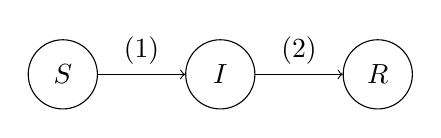
\begin{tikzpicture}
			\node[state] (S) {\(S\)};
			\node[state, right of = S] (I) {\(I\)};
			\node[state, right of = I] (R) {\(R\)};
			\draw (S) edge[above] node{(1)} (I)
			(I) edge[above] node{(2)} (R);
		\end{tikzpicture}
		\caption{A description of the SIR model formulated as a continuous-time Markov chain, including (top) the transition rates and (bottom) the corresponding transitions between states for an individual in a population.}
		\label{fig:sir_transition}
	\end{center}
\end{figure}

As a simple example, consider the susceptible-infected-recovered (SIR) model \citep{Allen_2017_PrimerStochasticEpidemic}, which is used to represent the spread of an infectious disease through a population where each individual is either susceptible (able to be infected), infected (and therefore infectious to susceptible individuals), or recovered (unable to be re-infected).
The transition rates are listed in \Cref{fig:sir_transition}, with the diagram indicating how an individual in the population moves through the three possible stages.
In the table, \(S\) denotes the number of susceptible individuals and \(I\) the number of infected individuals.
For a fixed population size \(M\), the number of recovered individuals \(R\) is given by \(R = M - S - I\), so we can formulate the stochastic model as 2-dimensional.
Let \(X_t \equiv \left(S_t,I_t\right)\) be the stochastic process, where \(S_t\) is the number of susceptible individuals and \(I_t\) the number of infected at time \(t\).
The state space of the process is then \(S = \setc{(s,i)}{s,i\in\set{0,1,\dotsc,M}, \, s + i \leq M}\).
There are two possible events that lead to a change in the state of the process: an infection of a susceptible individual, which occurs with a rate of \(\beta S_t I_t\) with \(S_t\) and \(I_t\) denoting the number of susceptible and infected individuals respectively at the time \(t\), and a recovery of an infected individual, which occurs with rate \(\gamma I_t\).
This is sufficient to fully describe the CTMC model.

As with stochastic differential equations, these models cannot in general be solved (in the sense of finding distributions across the state space at certain times, determining the long-term behaviour of the process, etc.) analytically, but can be simulated \citep{Gillespie_1977_ExactStochasticSimulation}, which is standard practice.
We summarise a method for simulating from a CTMC in \Cref{app:ctmc_sim}, which is used in examples later in this section.
The need for stochastic simulation leads to the same practical issues as we highlighted with SDEs; for complicated models, this is numerically inefficient and a large number of samples is needed for accurate inference.
However, these are approaches to approximating the behaviour of the CTMC that circumvent these computational difficulties.
Seminal work by \citet{Kurtz_1970_SolutionsOrdinaryDifferential,Kurtz_1971_LimitTheoremsSequences} showed that the stochastic evolution of certain CTMCs converge to the solutions to an ordinary and stochastic differential equation in the limit of infinite population size.
These processes are typically modelling a fixed population size and require that the transition rates only depend on the state of the process through the population-scaled proportion (e.g. the rates only depend on \(\frac1M X_t\) and not \(X_t\) directly for a population process \(X_t\) evolving with a fixed population size \(M\)).
Similar results for generalisations of these conditions do exist \citep{Pollett_1990_ModelInterferenceSearching}, however.
We briefly summarise these results---further details are provided in \Cref{app:epi_kurtz}---to which we can draw analogies with our own work.
Let \(X_t^{(M)}\) denote an \(n\)-dimensional population process, with each component taking values on the discrete set \(\set{0, 1, \dotsc, M}\).
The density process is then \(Y_t^{(M)} = \frac1M X_t^{(M)}\).
% In the limit of large population sizes, a deterministic ordinary differential equation and linear stochastic differential equation arise from certain population processes, despite these processes being discrete.
\citet{Kurtz_1970_SolutionsOrdinaryDifferential} showed that in the limit of large population size, \(M \to \infty\), the density process \(Y_t^{(M)}\) converges in probability to the deterministic trajectory \(Y_t^{(\infty)}\) that solves the ODE \citep{Kurtz_1970_SolutionsOrdinaryDifferential}
\begin{equation}\label{eqn:ctmc_ode}
	\dod{Y_t^{(\infty)}}{t} = Q\!\left(Y_t^{(\infty)}\right), \quad Y_0^{(\infty)} = \lim_{M\to\infty}\frac1M X^{(M)}_0,
\end{equation}
where \(Q\) is determined by the transition rates of the Markov chain and captures the average (macroscopic) behaviour of the density process.
The deterministic ODE \cref{eqn:ctmc_ode} is sometimes termed the \emph{fluid limit} of the population process.
Although the initial condition to \cref{eqn:ctmc_ode} is formally written as a limit, in practice \(Y_0^{(M)}\) can be specified directly.
\citet{Kurtz_1971_LimitTheoremsSequences} then further establishes a stronger result; that the stochastic variation of \(Y_t^{(M)}\) for large \(M\) can be described by the solution to a stochastic differential equation.
That is, the scaled process
\[
	Z_t^{(M)} = \sqrt{M}\left(Y_t^{(M)} - Y_t^{(\infty)}\right),
\]
which captures the deviation between the population process and the fluid limit, converges in distribution to the solution to the linear stochastic differential equation \citep{Kurtz_1971_LimitTheoremsSequences}
\begin{equation}
	\dif Z_t^{(\infty)} = \nabla Q\!\left(Y_t^{(\infty)}\right) Z_t^{(\infty)}\dif t + G\!\left(Y_t^{(\infty)}\right)\dif W_t, \quad Z_0^{(M)} = 0,
	\label{eqn:ctmc_sde}
\end{equation}
where the \(n\times n\) diffusion matrix \(G\) is also determined by the transition rates of the Markov chain, and \(W_t\) is a canonical \(n\)-dimensional Wiener process.
The diffusion term captures the microscopic behaviour resulting from individual transition events, and the uncertainty in this is parameterised with \(W_t\).
The diffusion limit \cref{eqn:ctmc_sde} is equivalent to the unscaled SDE
\begin{equation}
	\dif L_t^{(N)} = \left[Q\!\left(Y_t^{(\infty)}\right) + \frac{1}{\sqrt{N}} \nabla Q\!\left(Y_t^{(\infty)}\right)\left(L_t^{(N)} - Y_t^{(\infty)}\right)\right]\dif t + \frac{1}{\sqrt{N}}G\!\left(Y_t^{(\infty)}\right)\dif W_t,
	\label{eqn:ctmc_sde_lin_lim}
\end{equation}
which is then a linearisation of the nonlinear SDE
\begin{equation}
	\dif \hat{Y}^{(N)}_t = Q\!\left(\hat{Y}^{(N)}_t\right)\dif t + \frac{1}{\sqrt{N}}G\!\left(\hat{Y}_t^{(N)}\right)\dif W_t
	\label{eqn:ctmc_sde_lim_nonlin}
\end{equation}
about the deterministic limit \(Y_t^{(\infty)}\).
The diffusion limit \cref{eqn:ctmc_sde} (or \cref{eqn:ctmc_sde_lin_lim}) can be solved, and in the case of a fixed initial condition \(X_0\) follows a Gaussian distribution at any fixed time.
For large populations, the diffusion limit is used as an approximation to the population process that avoids the need for bulk simulation and has been shown to work remarkably well \citep{PollettEtAl_2010_ModellingPopulationProcesses}.

To illustrate the equations with an example, the SIR model is a density-dependent process.
The fluid limit is
\begin{equation}
	\dod{Y_t^{(\infty)}}{t} = \begin{bmatrix}
		-\beta Y_t^{(\infty,1)} Y_t^{(\infty, 2)} \\
		\beta Y_t^{(\infty,1)} Y_t^{(\infty, 2)} -\gamma Y_t^{(\infty, 2)}
	\end{bmatrix},
	\label{eqn:sir_fluid_limit}
\end{equation}
where \(Y_t^{(\infty)} \equiv \left(Y_t^{(\infty, 1)},Y_t^{(\infty, 2)}\right)^{\T}\) is the density process.
Here, the components of the density process are the proportion of the population susceptible and infected respectively.
The diffusion limit is the linear SDE
\begin{equation}
	\dif Z_t^{(\infty)} = \begin{bmatrix}
		-\beta X_t^{(\infty, 2)} & -\beta X_t^{(\infty, 1)}         \\
		\beta X_t^{(\infty, 2)}  & \beta X_t^{(\infty, 1)} - \gamma
	\end{bmatrix} Z_t^{(\infty)}\dif t + g\!\left(X_t^{(\infty)}\right)\dif W_t
	\label{eqn:sir_diff_limit}
\end{equation}
where
\[
	g\!\left(X_t^{(\infty)}\right) = \begin{bmatrix}
		\sqrt{\beta X_t^{(\infty, 1)} X_t^{(\infty, 2)}}  & 0                               \\
		-\sqrt{\beta X_t^{(\infty, 1)} X_t^{(\infty, 2)}} & \sqrt{\gamma X_t^{(\infty, 2)}}
	\end{bmatrix}.
\]
Solving \cref{eqn:sir_fluid_limit,eqn:sir_diff_limit} provides an alternative computation of the density process \(Y_t\)---by using \(Y_t^{(\infty)} + Z_t^{(\infty)} / \sqrt{M}\) as an approximation---that is valid in the sense of a limit.

We can draw analogies between these results and the SDE linearisation procedure in \Cref{ch:linear_theory}.
The fluid limit \cref{eqn:ctmc_ode} is analogous to the convergence of a small-noise SDE solution to the corresponding deterministic ODE solution, i.e. \(y_t^{(\epsilon)} \to y_t^{(0)}\) as \(\epsilon \downarrow 0\) in the notation of \Cref{ch:linear_theory}.
The diffusion limit in unscaled form \cref{eqn:ctmc_sde_lin_lim} is then comparable to the general linearisation \cref{eqn:linear_sde_inform} of a stochastic differential equation \cref{eqn:sde_y}, with \(\epsilon = 1/\sqrt{M}\).
However, a key difference is that in the SDE linearisation procedure, we start from a continuous state-space process and arrive at a continuous state-space process in the limit.
Whereas, in the diffusion limit, the converging process is on a \emph{discrete} state-space and the limit is on a continuous one.
We have also proven a stronger notion of convergence than in the original work of \citet{Kurtz_1971_LimitTheoremsSequences,Kurtz_1970_SolutionsOrdinaryDifferential}, by establishing bounds on the expectation (thus implying convergence in \(r\)th mean) in \Cref{thm:main}.
Regardless, our results and the diffusion limit for population processes are built around the same underlying linear stochastic differential equation, and so our practical results (i.e.\ stochastic sensitivity and the Gaussian mixture model algorithm) can be applied to characterise and approximate the solutions to these models.
In particular, we expect that the mixture model algorithm we have described may find a place in moderate-population compartmental models, where the population is large enough to be ``reasonably'' approximated by the continuous SDE equations, but small enough to exhibit non-Gaussian behaviour.

\begin{figure}
	\begin{center}
		\begin{subfigure}{0.49\textwidth}
			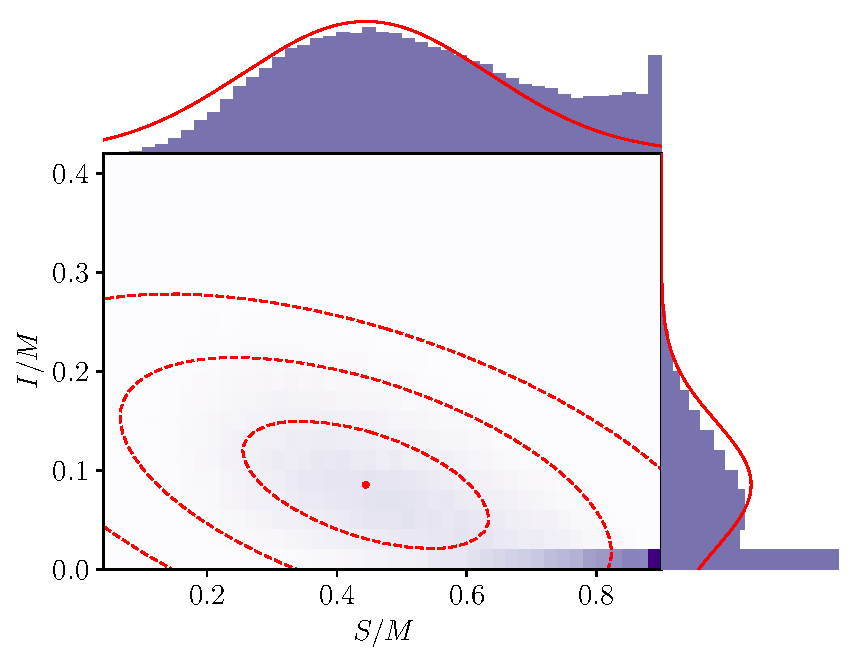
\includegraphics[width=\textwidth]{chp07_outlook/figures/sir/sir_pairwise_50}
			\caption{\(M = 50\)}
			\label{fig:sir_gauss_rels_1}
		\end{subfigure}
		\begin{subfigure}{0.49\textwidth}
			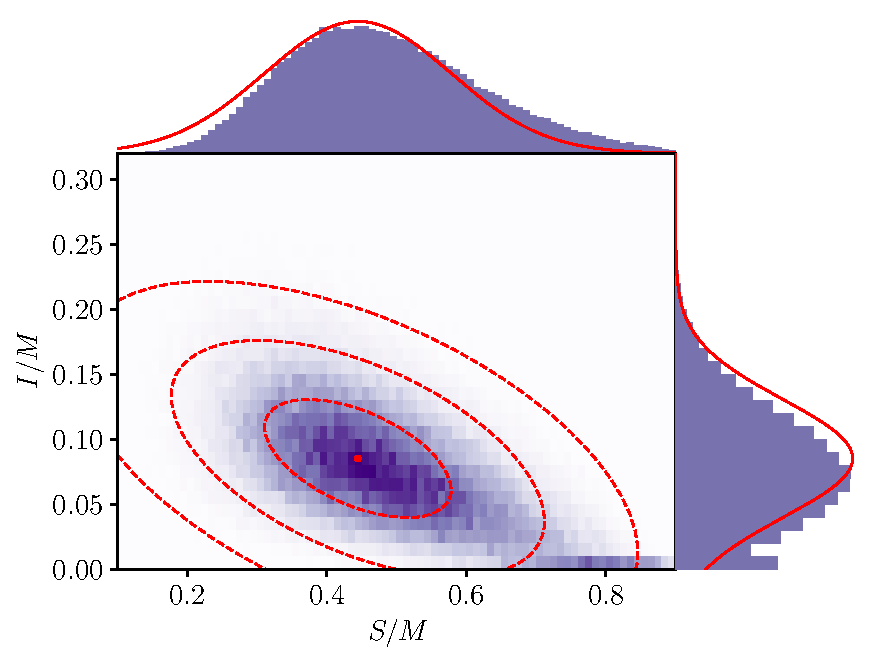
\includegraphics[width=\textwidth]{chp07_outlook/figures/sir/sir_pairwise_100}
			\caption{\(M = 100\)}
			\label{fig:sir_gauss_rels_2}
		\end{subfigure}
		\begin{subfigure}{0.49\textwidth}
			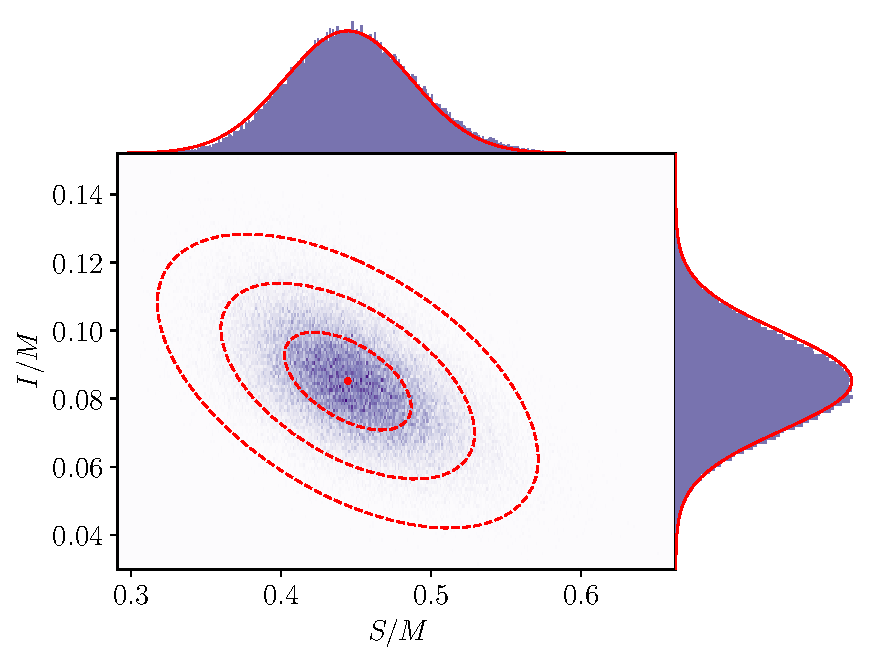
\includegraphics[width=\textwidth]{chp07_outlook/figures/sir/sir_pairwise_1000}
			\caption{\(M = 1000\)}
			\label{fig:sir_gauss_rels_3}
		\end{subfigure}\begin{subfigure}{0.49\textwidth}
			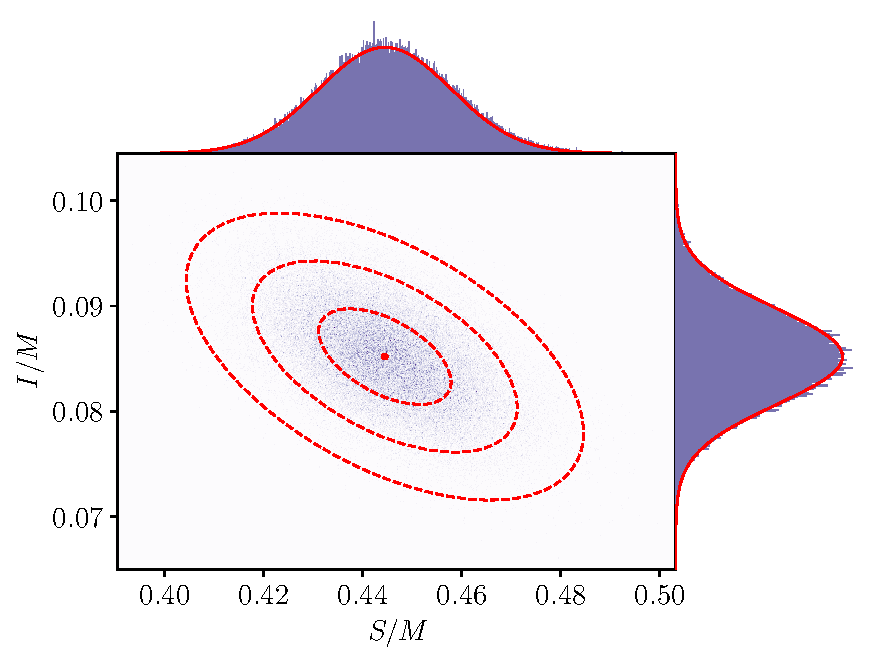
\includegraphics[width=\textwidth]{chp07_outlook/figures/sir/sir_pairwise_10000}
			\caption{\(M = 10000\)}
			\label{fig:sir_gauss_rels_4}
		\end{subfigure}
		\caption{Histograms of Monte-Carlo simulations of the density process for the SIR model (with marginal plots on each axis), and the probability density function of the corresponding solution to the diffusion limit \cref{eqn:sir_diff_limit} plotted in red.
			The parameters are \(\beta = 1.2\) and \(\gamma = 0.8\), and each sample path is initialised with 10\% of the population infected and simulated up to \(t = 5\).
			The bins are chosen to reflect the state-space \(\set{0, 1/M, 2/M, \dotsc, 1}\) of the density process.}
		\label{fig:sir_gauss_rels}
	\end{center}
\end{figure}

We shall now demonstrate some of these calculations, to highlight how our results are consistent with those in the population process modelling space and postulate future application of stochastic sensitivity and our mixture model algorithm.
In \Cref{fig:sir_gauss_rels}, we show histograms of \(10000\) realisations of the population-scaled SIR model (so realisations of the density process) for four different population sizes.
We set the parameters \(\beta = 1.2\) and \(\gamma = 0.8\), initialised each process with 10\% of the population infected and the remaining susceptible (so \(X_0^{(M)} = \left(0.1M, 0.9M\right)^{\T}\)) and show each realisation at \(t = 5\) time units.
We also compute the Gaussian solution to the diffusion limit, using the \citet{Mazzoni_2008_ComputationalAspectsContinuous} method for rapid computation of the moments of the solution to \Cref{eqn:ctmc_sde_lin_lim}, and show resulting density as contours on the joint histograms and by plotting the marginal PDFs on each axis.
As the population size \(M\) increases, the Gaussian approximation provides a closer representation of the empirical distribution of the samples.
This should be compared with \Cref{fig:sine_hists,fig:1d_mult_hists}, where we verified heuristically that the solutions to small-noise SDEs approached the Gaussian solution of the linearisation.
It is also evident in \Cref{fig:sir_gauss_rels} that the boundaries limit the validity of the Gaussian approximation: the density process is restricted to \([0, 1]\) with an absorbing state at \(0\) that results in the accumulation of probability mass seen in the histograms.
Such boundary problems are common in epidemiological and biological models, e.g. the early spread of a disease through a population is often of interest, and the inability of the diffusion limit to appropriately account is as a significant limitation.
We discussed in \Cref{sec:disc_bc} the boundary complication in reference to our SDE linearisation framework and suggested that appropriately accounting for boundary conditions and absorbing states would be a valuable avenue for future work.
Any developments to this end, whether that be a modification to the linearised SDE itself or an adjustment to the solution PDF, would also be useful for the diffusion limit of a CTMC.


\begin{figure}
	\begin{center}
		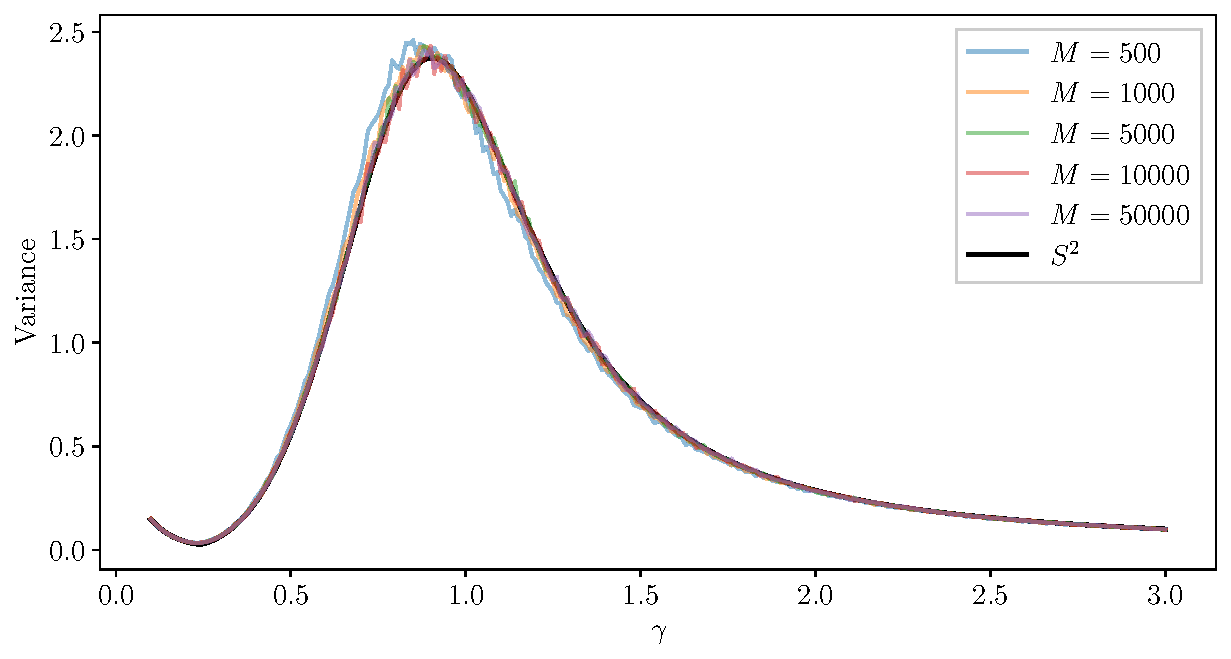
\includegraphics[width=\textwidth]{chp07_outlook/figures/sir/sir_s2_R0}
		\caption{The stochastic sensitivity value (in black) of the SIR diffusion limit \cref{eqn:sir_diff_limit} at time \(t = 5\) and from the fixed initial condition of 10\% of the population infected, for \(\beta = 1\) and varying \(\gamma\).
			The maximum projection of the sample covariance matrix (in various colours) for \(1000\) stochastic simulations of the discrete population process over the same time interval is included.}
		\label{fig:sir_s2}
	\end{center}
\end{figure}

Next, we compute stochastic sensitivity for a density-dependent CTMC using the diffusion limit.
We can compute the covariance matrix of the solution to the diffusion limit \cref{eqn:ctmc_sde}, which satisfies the covariance differential equation \cref{eqn:pi_ode} from \Cref{ch:linear_theory} with \(Q\) in place of \(u\) and \(g\) in place of \(\sigma\).
Then, the stochastic sensitivity value is calculated by taking the operator norm, using this matrix in place of \(\Sigma_0^t\) in \Cref{thm:s2_calculation}.
In \Cref{fig:sir_s2}, we plot the computed stochastic sensitivity for the SIR model against the corresponding empirical value (the operator norm of the sample covariance matrix) from 1000 realisations of the population process, for varying population size \(M\).
We have fixed \(\beta = 1\) and varied \(\gamma\).
For each parameter value, we again initialised with 10\% of the population infected and considered up to \(T = 4\).
The variance is of the density process, but can be rescaled to that of the original population process by multiplying by \(M^2\).
Even for a small population size, the stochastic sensitivity provides a reliable indication of the variation in the population process, and therefore can serve as a tool in analysing these models.
This is not dissimilar to the work of \citet{PollettEtAl_2010_ModellingPopulationProcesses}, who suggest that the covariance matrix of the solution to the diffusion limit measures the ``unexplained variation'' in using the fluid limit alone to approximate the fully stochastic process.
One advantage of stochastic sensitivity is that it provides a single number, by performing a dimension reduction, which avoids ambiguity in higher dimensions and provides a similar diagnosis for population processes.


\begin{figure}
	\begin{center}
		\begin{tabular}{|c|c|c|}
			\hline
			Transition & Event                                               & Rate \(\lambda_i\)                                               \\ \hhline{|=|=|=|}
			(1)        & \(\left(S, E\right) \to \left(S-1, E+1\right)\)     & \(\left(\beta_I SI + \beta_H SH + \beta_F SF\right) / N\)        \\ \hline
			(2)        & \(\left(E, I\right) \to \left(E - 1, I + 1\right)\) & \(\alpha E\)                                                     \\ \hline
			(3)        & \(\left(I, H\right) \to \left(I - 1, H + 1\right)\) & \(\gamma_H \theta_1 I\)                                          \\ \hline
			(4)        & \(\left(H, D\right) \to (H - 1, D + 1)\)            & \(\gamma_{dh}\delta_2 H\)                                        \\ \hline
			(5)        & \(\left(D\right) \to \left(D - 1\right)\)           & \(\gamma_f D\)                                                   \\ \hline
			(6)        & \(\left(I\right) \to \left(I - 1\right)\)           & \(\gamma_i\left(1 - \theta_1\right)\left(1 - \delta_1\right) I\) \\ \hline
			(7)        & \(\left(I, D\right) \to \left(I - 1, D + 1\right)\) & \(\delta_1 \left(1 - \theta_1\right) \gamma_d I\)                \\ \hline
			(8)        & \(\left(H\right) \to \left(H - 1\right)\)           & \(\gamma_{ih}\left(1 - \delta_2\right)H\)                        \\ \hline
		\end{tabular} \\
		\vspace{2mm}
		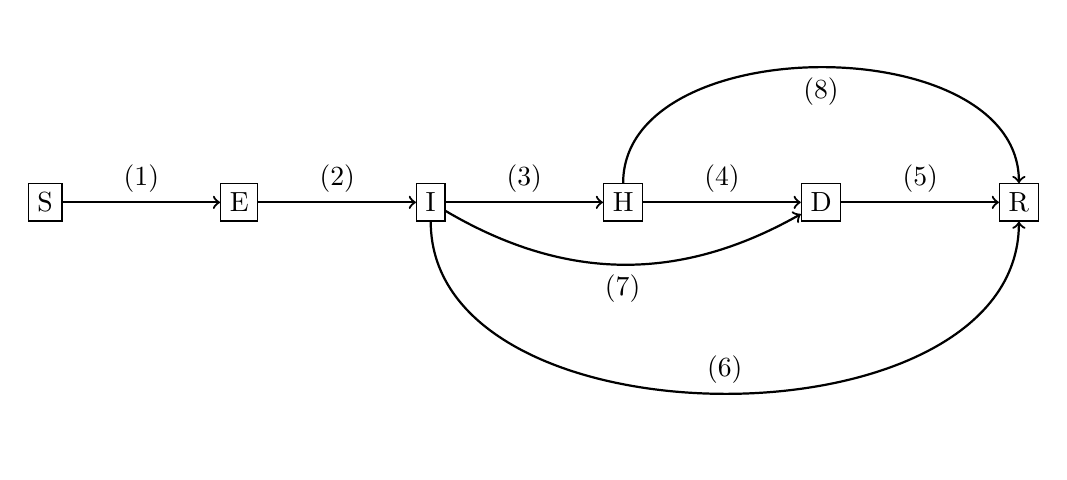
\begin{tikzpicture}
			\node (S) [draw] {S};
			\node (E) [draw, right=of S] {E};
			\node (I) [draw, right=of E] {I};
			\node (H) [draw, right=of I] {H};
			\node (F) [draw, right=of H] {D};
			\node (R) [draw, right=of F] {R};
			\path[->,thick] (S) edge[above] node{(1)}  (E)
			(E) edge[above] node{(2)} (I)
			(I) edge[above] node{(3)} (H)
			(H) edge[above] node{(4)} (F)
			(F) edge[above] node{(5)} (R)
			(I) edge[bend right=90, above] node{(6)} (R)
			(I) edge[bend right, below] node{(7)} (F)
			(H) edge[bend left=90, below] node{(8)} (R);
		\end{tikzpicture}
		\caption{Transition probabilities of the Ebola model of \citet{LegrandEtAl_2007_UnderstandingDynamicsEbola}.}
		\label{fig:ebola_transition}
	\end{center}
\end{figure}

Finally, we will demonstrate the computation of the Gaussian approximation on a 5-dimensional model.
The Gaussian approximations become particularly useful in high-dimensions, where the number of stochastic samples to make accurate inferences scales poorly.
We consider a 5-dimensional model for the spread of Ebola, used in a case study by \citet{LegrandEtAl_2007_UnderstandingDynamicsEbola} on two particular outbreaks in the Democratic Republic of Congo and Uganda.
This model is far more complicated than the SIR example: the transition events and a diagram corresponding to the evolution of an individual through the stages of the infection are provided in \Cref{fig:ebola_transition}.
Similar to the SIR model, an individual the population is in one of six possible stages: susceptible (\(S\)), exposed to the infection but not yet infectious (\(E\)), infectious to susceptible individuals (\(I\)), hospitalised (\(H\)), deceased with a traditional burial (\(D\)), and removed from the population and no longer infectious or susceptible (\(R\)).
We choose this model specifically as the study by \citet{LegrandEtAl_2007_UnderstandingDynamicsEbola} provides values for all the involved parameters that are fitted using an actual outbreak of Ebola in 1995 in the Democratic Republic of Congo, immediately providing us with a physically relevant model. The population size is fixed at \(M = 200000\) \citep{DowellEtAl_1999_TransmissionEbolaHemorrhagic} and the initial condition is \(X_0 = (0, 0, 3, 0, 0)\) \citep{KhanEtAl_1999_ReemergenceEbolaHemorrhagic} in accordance with the 1995 outbreak.
The model by \citet{LegrandEtAl_2007_UnderstandingDynamicsEbola} is then formulated as a 5-dimensional CTMC \(Xt \equiv \left(S_t, E_t, I_t, H_t, D_t\right)^{\T}\), where each component tracks the number of individuals in each of the compartments and the number of removed individuals at any time given by \(R_t = M - S_t - E_t - I_t - H_t - D_t\).
Since we only provide a demonstration of the computation involved, rather than exploring this example in detail, further details are left to \Cref{app:ebola}.
We take the parameter values from \citet{LegrandEtAl_2007_UnderstandingDynamicsEbola}, who combined values estimated from other studies \citep{BwakaEtAl_1999_EbolaHemorrhagicFever,DowellEtAl_1999_TransmissionEbolaHemorrhagic,KhanEtAl_1999_ReemergenceEbolaHemorrhagic,NdambiEtAl_1999_EpidemiologicClinicalAspects,RoweEtAl_1999_ClinicalVirologicImmunologic} with their own maximum likelihood estimates using morbidity data.
These parameter values are provided in \Cref{tab:ebola_param_vals} in \Cref{app:ebola}.

The CTMC with the rates described in \Cref{fig:ebola_transition} is density-dependent, meaning that the fluid and diffusion limits hold.
We provide the ODE and SDE in \Cref{app:ebola}, for which we can solve jointly by again using the Mazzoni method, which scales well with the increased dimension as the algorithm relies primarily on matrix calculations.

In \Cref{fig:ebola_marginals}, we have generated 10000 realisations of the CTMC model after 20 weeks and plotted empirical histograms of the population-scaled counts.
To visualise the 5-dimensional distribution of these realisations, we have plotted joint histograms of each pair of components on the off-diagonals. On the diagonal, we have included histograms of each component of the realisations.
We also compute the Gaussian solution to the diffusion limit and overlay contours of the joint marginal PDFs corresponding to each pair of components, and the PDF itself on each single-variable marginal.
Since the population size in this example is large (\(M = 200000\)), the Gaussian approximation is reasonable even in this high-dimensional setting.
However, there are small departures from Gaussianity, including skewness in the single-variable marginals and nonlinear correlations in the joint density.
The mixture model algorithm may have potential to capture these features and provide a more accurate approximation.
This would require further development of the algorithm, however, including appropriate handling of the boundary conditions (i.e.\ note the proximity of the component distributions to \(0\)).
Nonetheless, we expect that the mixture model will provide a computationally efficient alternative to stochastic simukation of high dimensional CTMC models, and this has much potential in this area.
% This is also being pursued as future work from this areagcc

We have only provided a short overview of the diffusion limit, drawn analogies and complemented this discussion with two examples.
These connections are highly promising, however, and suggest that stochastic sensitivity and our mixture model, with further refinement, has applications across a far broader range of models than the stochastic differential equations we originally worked with.
The mixture model in particular could provide an approximate method for solving complicated and high-dimensional stochastic models without simulation, which is an area of high interest in the fields of biological modelling \citehere.
Moreover, whereas the diffusion limit and the inference on the model it provides is well used across applications \citep[e.g.]{PollettEtAl_2010_ModellingPopulationProcesses,Pollett_1990_ModelInterferenceSearching}, these ideas are novel in the dynamical systems and stochastic differential equations
settings.
By establishing connections between our results and those for discrete stochastic models, we can provide tools from either field in new situations and contexts, bridging a gap between two otherwise disparate fields.

\begin{landscape}
	\begin{figure}
		\centering
		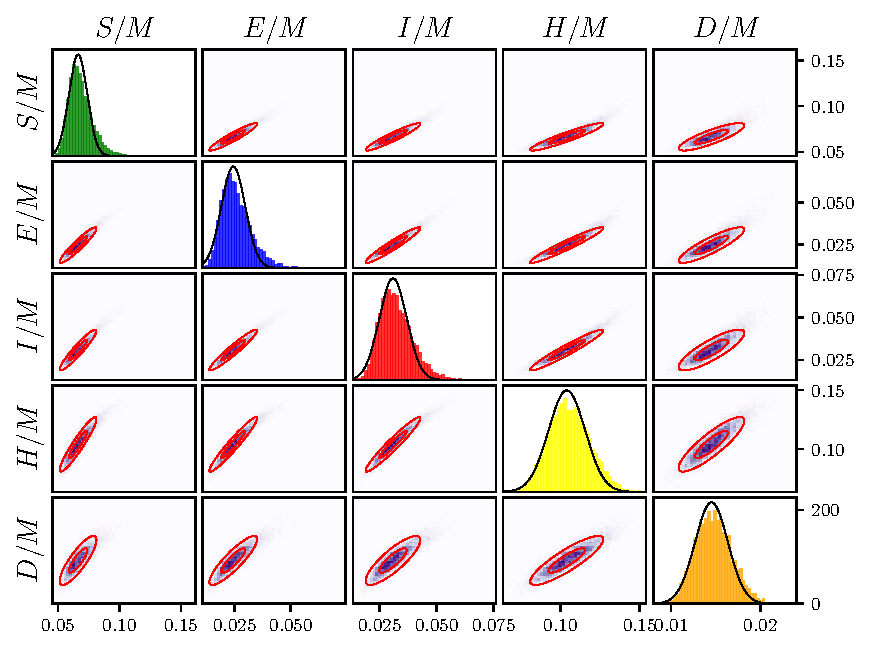
\includegraphics[width=\textheight]{chp07_outlook/figures/seihfr/seihfr_marginals_gaussian}
		\caption{Histograms of 100000 realisations of the 5-dimensional Ebola model by \citet{LegrandEtAl_2007_UnderstandingDynamicsEbola}, after 20 weeks.
			Each row and column corresponds to one of the 5 components of the process, with the off-diagonal plots showing the joint bivariate histograms of each pair of components and the diagonal entries showing the single-component marginals.
			Overlaid in red on each histogram are the contours (for the joint histograms) or probability density functions (for the single-component histograms) of the corresponding marginals of the Gaussian approximation that solves the diffusion limit.}
		\note{I will tweak this plot to include axis ticks next week; my first run through of the full thesis will be to bring all plots up to scratch and ensure that they are consistent.}
		\label{fig:ebola_marginals}
	\end{figure}
\end{landscape}

% \subsection{Observation-driven modelling}
% \note{Possible advantages levied by the expressions for the Gaussian approximation written in terms of the flow-map.}
% \td{Perhaps find a better section name. Still need to check that there is enough here to warrant a whole dedicated subsection}


% \citet{Sura_2003_StochasticAnalysisSouthern} analyse the dynamics of sea-surface winds across the Southern Ocean by constructing a stochastic differential equation \emph{empirically}.
% The drift and diffusion of a stochastic differential equation can be defined as statistical quantities, by taking averages over the solution distribution.
% For instance, given an autonomous stochastic differential equation
% \begin{equation}\label{eqn:auto_sde}
% 	\dif x_t = A\!\left(x_t\right)\dif t + B\!\left(x_t\right)\dif W_t,
% \end{equation}
% the drift \(A\) and diffusion \(B\) satisfy \citehere
% \begin{align*}
% 	A(x)          & = \lim_{\delta t \to 0}\frac{1}{\delta t}\avg{x_{t + \delta t} - x}                                                   \\
% 	B(x)B(x)^{\T} & = \lim_{\delta t \to 0}\frac{1}{\delta t}\avg{\left(x_{t + \delta t} - x\right)\left(x_{t + \delta} - x\right)^{\T}},
% \end{align*}
% where the expected values are taken over all trajectories solving \cref{eqn:auto_sde} with \(x_t = x\).

% In deriving expressions for the solution to a linearised stochastic differential equation, we provided explicit expressions (\Cref{cor:limit_moments}) for the mean and covariance of the linearised solution written in terms of just the flow map and diffusion matrix \(\sigma\).
% With specification of \(\sigma\), the first two moments of the solution to the linearised SDE can be computed by approximating the appropriate spatial derivatives of the flow map \(F\).
% That is, without the need to determine the velocity field as an intermediate step.



%%% DUMP OF COMMENTS FROM PAPER - MOST HAS ALREADY BEEN WORKED INTO THE ABOVE
% This result extends the convergence bound on the Kullback-Leibler divergence by Sanz-Alonso and Stuart \cite{Sanz-AlonsoStuart_2017_GaussianApproximationsSmall} to an explicit bound on the convergence of all moments of the difference between the exact SDE solution and the approximation, and further establishes the exact Gaussian distribution in the small-noise limit.
% Our bound is verified numerically by plotting the first four raw moments of the distance between the true noise-scaled solution and the linearised solution (see \Cref{fig:gamma_z_valid}).
% The results, plotted across three orders of magnitude of the small noise parameter, match our theoretical prediction exactly.

% In addition, we described a framework in which uncertainty in deterministic models can be ascribed without the need for expensive stochastic simulation, and purely from understanding of the initial condition and deterministic solution dynamics.
% We illustrated how the Gaussian limit reflects the time-evolution of uncertainty (see \Cref{fig:time_evol}), even when the true uncertainty distributions are themselves non-Gaussian.

% Data assimilation is a framework for improving uncertainties in predictions by combining model forecasts with observational data, accounting for error in both, and uncertainty quantification refers to the broader goal of capturing the uncertainty inherent in prediction \cite{BudhirajaEtAl_2019_AssimilatingDataModels,Jazwinski_2014_StochasticProcessesFiltering,LawEtAl_2015_DataAssimilationMathematical,ReichCotter_2015_ProbabilisticForecastingBayesian}.
% The Gaussian limit here provides a characterisation of model uncertainty, and may therefore be useful in data assimilation and uncertainty quantification.
% The linearisation of the stochastic differential equation \cref{eqn:sde_y} used to construct the Gaussian approximation has been employed in data assimilation, e.g. in the continuous time continuous state-space extended Kalman filter \cite[\S 9]{Jazwinski_2014_StochasticProcessesFiltering}. The convergence analysis of this paper could contribute a new term, estimating the error due to linearisation, to the \emph{forecast uncertainty} covariance matrix employed in these extended Kalman filters.


% % The multiplicative noise is captured by the Gaussian approximation by evaluating \(\sigma\) along the deterministic reference trajectory.
% % The Gaussian uncertainties capture both the model dynamics, and any multiplicative or spatiotemporal dependence in the uncertainty, through specification of \(\sigma\).
% We therefore present a highly flexible framework that can capture any prior knowledge of non-uniform uncertainty that arises from modelling or experimental considerations.

% \td{Very brief comparison to Sanz-Alonso}
% Our bound in \cref{eqn:main_ineq} is comparable to that placed on the Kullback-Leibler divergence by \citet{Sanz-AlonsoStuart_2017_GaussianApproximationsSmall}; the Kullback-Leibler between the linearised solution and the SDE solution is bounded by a sum of the Kullback-Leibler divergence in the initial condition and a constant term scaled by \(\epsilon\).
% Our bound \cref{eqn:main_ineq} on the strong error between the SDE solution and the linearisation consists of error in the initial condition, a constant scaling with \(\epsilon\), and an additional term involving both the initial uncertainty and \(\epsilon\).



% An initial study into the impact of uncertainty of one such method -- the finite-time Lyapunov exponent -- has already been performed using stochastic sensitivity \cite{Balasuriya_2020_UncertaintyFinitetimeLyapunov}, albeit in only two-dimensions and without knowledge that the limiting distribution is Gaussian.

% \td{In the following, be careful about mentioning the higher order terms. We have only provided an explicit bound for the first-order expansion, whereas the small noise proofs are up to arbitrary order. But our justification for looking at only the first order terms is the computability and use of Gaussian approximations elsewhere - higher order terms satisfy SDEs that cannot be solved in general and require higher order derivatives. This is possibly better placed in the introduction.}
% The Gaussian approximation presented here arises as the leading order term in a power series expansion of the SDE solution in terms of the noise scale parameter \(\epsilon\) \cite{Blagoveshchenskii_1962_DiffusionProcessesDepending}.
% A further extension would be to explore the higher-order terms in such an expansion, which could lead to a practical framework for constructing higher-order characterisations and approximations of the stochastic solution.
% However, the higher-order terms are known to be individually non-Markovian, and satisfy non-linear SDEs for which the solution is not expected to be analytically available \cite{Blagoveshchenskii_1962_DiffusionProcessesDepending}.

% In this paper, we have assumed throughout that the initial condition \(x\), from which both the stochastic differential equation and the deterministic flow map evolves from, is \emph{certain} (i.e. not a random quantity).
% However, in practice there is uncertainty associated with the initial state which should also be accounted for.
% The bound in \Cref{thm:main} is independent of the initial condition, suggesting that the required extension of the theoretical result is straightforward.
% This extension will broaden our framework, allowing for uncertainties in \emph{both} the initial state and the time-evolution of the model to be characterised at once in a precise sense.

% Similarly, we assume that the reference deterministic model \cref{eqn:ode_det} for the evolution of the state variable is ``correct'' and known exactly, in that in the absence of any noise (i.e. \(\varepsilon = 0\)), the SDE model \cref{eqn:sde_y} reduces to the deterministic \cref{eqn:ode_det}.
% The Gaussian characterisation is computed from knowledge of either the driving vector field or the solution data itself, i.e. the flow map.
% However, these components of the deterministic model may not be known exactly, e.g. from solving \cref{eqn:ode_det} numerically, interpolation error, etc.
% There is a need to extend the theory presented here to account for this case; to, for instance, establish a bound in the error between the SDE solution and the limiting Gaussian, as in \Cref{thm:main}, if the Gaussian distribution is constructed from an ``incorrect'' deterministic model.
% Both of these theoretical extensions, to uncertain initial conditions and incorrect deterministic dynamics, are currently being pursued.


% \td{Shorten the following and meld into discussion}
% Here, we briefly discuss some anticipated applications of this work across a wide range of fields, including climate and ocean modelling, data assimilation and Lagrangian coherent structures.

% To ascribe uncertainties directly onto the deterministic model, we assume that the diffusivity matrix \(\sigma\) is specified \textit{a priori}, to capture any known multiplicative noise effects.
% There are methods for estimating \(\sigma\) directly from observed data, e.g. the Bayesian inference approach of \cite{YingEtAl_2019_BayesianInferenceOcean} or via statistical estimation as in \cite{CotterPavliotis_2009_EstimatingEddyDiffusivities}, which can be used in our framework.
% In particular, \cite{YingEtAl_2019_BayesianInferenceOcean} relies upon computationally expensive numerical approximations to compute the likelihood of each trajectory, whereas from this paper we have a potentially more efficient computation, using the analytically available Gaussian limit.
% Coupling these approaches with the approximation here could provide a complete and practical framework to characterise the uncertainty in the flow by efficiently estimating the (multiplicative) diffusion from observed trajectory data.


% Moreover, most traditional LCS measures are completely deterministic measures, not accounting for any uncertainty in the driving velocity field, and the sensitivity of these methods to such uncertainty has not been investigated in detail.
% The robustness of several LCS methods to stochastic noise has recently been explored in \cite{BadzaEtAl_2023_HowSensitiveAre}, but via stochastic simulation and summary statistics.
% In this paper we have presented a theoretical result for characterising Lagrangian trajectory uncertainty, which can be used to perform a purely theoretical analysis of such sensitivity in LCS computations.
% An initial study into the impact of uncertainty of one such method -- the finite-time Lyapunov exponent -- has already been performed using stochastic sensitivity \cite{Balasuriya_2020_UncertaintyFinitetimeLyapunov}, albeit in only two-dimensions and without knowledge that the limiting distribution is Gaussian.

% % There are several methods for computing the flow map gradient directly from observed tracer data, in the context of calculating finite-time Lyapunov exponents (FTLEs) \cite{Leung_2013_BackwardPhaseFlow, RabenEtAl_2013_ComputationFinitetimeLyapunov}.
% % Another question would be whether the techniques of estimating the flow map gradient in the LCS literature can be coupled with a data assimilation scheme, by using the characterisation of the Gaussian approximation in terms of solely the flow map gradients.


% % Speaking more generally, determining the structure of the model error
% % More complications arise if this model error is state (e.g. position) dependent, which is expected in many contexts \cite{Bishop_2019_DataAssimilationStrategies}.
% % The work here presents a framework for computing a state-dependent model error covariance matrix entirely from the deterministic model dynamics.
% % \td{Are we implicitly extending EKF to state-dependent covariances?}

% % As an alternative, there are recent DA approaches that directly use coherent structures \cite{MacleanEtAl_2017_CoherentStructureApproach, Schlueter-KuckDabiri_2019_ModelParameterEstimation}, for which stochastic sensitivity could be applied to use coherent structures that reflect model certainty.

% Stochastic sensitivity provides a novel method for extracting Lagrangian coherent structures (LCSs) \cite{BalasuriyaEtAl_2018_GeneralizedLagrangianCoherent, HadjighasemEtAl_2017_CriticalComparisonLagrangian} from fluid flow, by considering regions with uncertainty (as measured by the stochastic sensitivity field) below a prescribed threshold.
% Whereas the original formulation in \cite{Balasuriya_2020_StochasticSensitivityComputable} was restricted to two-dimensional flows, here we have an extension of the LCS extraction scheme to arbitrary dimensions.

% LCS extraction has recently been used as a means of dimension reduction in data assimilation schemes \cite{MacleanEtAl_2017_CoherentStructureApproach,MorzfeldEtAl_2018_FeaturebasedDataAssimilation,Schlueter-KuckDabiri_2019_ModelParameterEstimation}.
% Through stochastic sensitivity, we have a method for extracting coherent regions that directly reflect model uncertainty, and so may be applicable in these DA schemes.


% The original formulation of stochastic sensitivity in \cite{Balasuriya_2020_StochasticSensitivityComputable} presented a novel approach to characterising coherence in unsteady flows in the presence of Eulerian noise in 2D flows.
% The potential of this approach has only just begun to be explored \cite{BadzaEtAl_2023_HowSensitiveAre}.\lb{Missing a sentence or two here on how SS can quantify uncertainty in LCS measures, including the citation \cite{Balasuriya_2020_UncertaintyFinitetimeLyapunov}. Also, worth mentioning LCS extraction in 3D and beyond with SS?} With the additional knowledge that the limiting distribution is Gaussian, the corresponding error in the FTLE field could be calculated in a statistically rigorous way, e.g. via formal confidence intervals.
% This approach could also be extended to other methods for detecting Lagrangian coherent structures, since many of these use the deterministic flow map over a finite time interval \cite{BalasuriyaEtAl_2018_GeneralizedLagrangianCoherent, HadjighasemEtAl_2017_CriticalComparisonLagrangian}.

% The non-Gaussianity can be approximated
% For instance, Gaussian mixture models are an analytically tractable framework for combining multiple correlated Gaussian distributions to approximate a non-Gaussian one, and there has been recent interest in applying this approach to stochastic differential equations \citehere. %\cite{SunEtAl_2022_DataDrivenAdaptive, ??}.
% \td{Talk very briefly about Jack's idea}

% \subsection{Old bits}
% Discussion:

% The main contributions of this manuscript are to
% \begin{enumerate}[label=\arabic{*}.]
%  \item  Extend SS to any dimension and provide exact Gaussian result
%  \item Provide
%  \item Should honorably mention  and their KL divergence bound here; ours is to bound all moments and handle multiplicative noise.
%  \item Our method is verified numerically for the first four moments of an sde, and ...
%  \item Should include the differential form in this paper and then link it here, as your method only requires simulation of two ODEs
% \end{enumerate}

% Extensions:

% \begin{enumerate}[label=\arabic{*}., ref=(\roman{*})]
%  \item Discuss extension to incorrect initial condition and to incorrect deterministic dynamics.
% \end{enumerate}

% Future applications:

% \begin{enumerate}[label=\arabic{*}., ref=(\roman{*})]
%  \item Comment that as cited in Discussion, the approximation of the solution of the FPE is of constant interest. This section tries to identify some contemporary areas in which this paper may contribute.
%  \item Discuss stoch param, DA here
%  \item Also classic multiscale methods? It's not clear whether Liam's result can be applied to stochastic averaging or homogenization, but worth considering.
% \end{enumerate}

% Gaussian approximations of stochastic differential equation solutions are employed across a broad range of applications, but there is ambiguity about the handling of the diffusion coefficients \citehere and the mathematical validity of using the approximation \cite{Sanz-AlonsoStuart_2017_GaussianApproximationsSmall}, in particular when the equation is non-autonomous.
% This paper has presented a rigorous justification of a Gaussian approximation for a fully non-autonomous stochastic differential equation with multiplicative noise.

% This work fits in with recent interest in stochastic parameterisation as a means to account for unresolved subgrid effects in climate and oceanographic modelling \cite{BernerEtAl_2017_StochasticParameterizationNew}.

% \td{The punchline - the expression of the approximation only in terms of the model dynamics - we can take \textit{any} deterministic model and add noise}
% Although the stochastic differential equation in \cref{eqn:sde_y} was used to theoretically formulate and justify the Gaussian approximation, the final statement of the approximation in \cref{eqn:y_t_gauss} makes no reference to this equation, other than in the specification of the diffusion matrix \(\sigma\).
% This is the key contribution of this work; we have described a framework to take a deterministic model and ascribe Gaussian uncertainties \emph{entirely} from the model itself.
% The framework can also address multiplicative noise through specification of \(\sigma\), which is necessary to capture non-Gaussianity (e.g. \cite{SuraEtAl_2005_MultiplicativeNoiseNonGaussianity})\lb{I don't like saying ``non-Gaussianity'' here, since the whole point of this paper is Gaussian approximations. The cited article explores how non-Gaussian statistics can arise from a linear model with multiplicative noise, as opposed to a non-linear model with additive noise.} and anisotropy (e.g. \cite{KamenkovichEtAl_2015_PropertiesOriginsAnisotropic}) in the unresolved processes.

% The default choice of \(\sigma \equiv I\) addresses a generic situation \citehere, and there are methods for estimating \(\sigma\) directly from observed data, e.g. \citehere or the Bayesian inference approach of \cite{YingEtAl_2019_BayesianInferenceOcean}.
% Coupling these approaches with the approximation here could provide a complete and practical framework for constructing a Gaussian approximation from observed trajectory data only, without the need to directly specify the diffusion matrix \emph{a priori}.

% % Conversely, such approaches for estimating eddy diffusivity and particle dispersion rely upon numerical solutions.
% % For example, the Bayesian approach of \cite{YingEtAl_2019_BayesianInferenceOcean} numerically solves the Fokker-Planck equation to compute the likelihood of the observed drifter data for each proposed diffusivity tensor, which requires significant computational overhead.
% % Using the Gaussian approximation, computed using , we have a likelihood function that can be used directly in Bayesian inference methods.



% % The setting here is more general than that covered by Sanz-Alonso and Stuart \cite{Sanz-AlonsoStuart_2017_GaussianApproximationsSmall}, in that the noise is permitted to be multiplicative and non-stationary through a diffusion matrix \(\sigma\) varying spatiotemporally.

% % The work here is strongly related to Freidlin-Wentzell large- and moderate-deviation theory \cite{FreidlinWentzell_1998_RandomPerturbationsDynamical}, which aims to .

% There are many anticipated extensions and applications of this work in a wide range of fields, particularly in ocean and atmospheric modelling, data assimilation and Lagrangian coherent structures.

% An immediate extension of this work is to consider uncertainty about the initial condition, which can occur in both \td{something} and iterative schemes.
% \td{Talk about extension to uncertain initial conditions}
% The approximation would no longer be Gaussian, and instead can be expressed as the independent sum of the scaled initial condition and the zero-mean Gaussian approximation presented here.
% Providing that the distribution of the initial condition is known analytically, or can be sampled from, this means ...
% Such a formulation would allow for iterative schemes to be constructed, such as a those employed in the data assimilation setting, in which the uncertainty and approximation is progressively updated over discrete time steps.


% The original formulation of stochastic sensitivity in \cite{Balasuriya_2020_StochasticSensitivityComputable} presented a novel approach to characterising coherence in unsteady flows in the presence of Eulerian noise in 2D flows.
% The potential of this approach has only just begun to be explored \cite{Balasuriya_2020_StochasticSensitivityComputable, BadzaEtAl_2023_HowSensitiveAre}, and the extension to arbitrary dimension presented here allows this new tool to be immediately applied in three-dimensional flows.

% \td{If this part is included at all, needs to be stated in vaguer terms.}
% In \cite{Balasuriya_2020_UncertaintyFinitetimeLyapunov}, the original formulation of stochastic sensitivity is used to calculate an error for the finite-time Lyapunov field.
% % Given an initial condition \(x_0 \in \R^2\), the norm of the uncertainty in the final location is bounded by \(\epsilon^2\sqrt{S^2\left(x_0\right)}\),
% % This bound then leads to a computable formula for the error in the value of the FTLE along the deterministic trajectory starting from \(x_0\).
% With the additional knowledge that the limiting distribution is Gaussian, the corresponding error in the FTLE field could be calculated in a statistically rigorous way, e.g. via formal confidence intervals.
% This approach could also be extended to other methods for detecting Lagrangian coherent structures, since many of these use the deterministic flow map over a finite time interval \cite{AllshousePeacock_2015_LagrangianBasedMethods, BalasuriyaEtAl_2018_GeneralizedLagrangianCoherent, HadjighasemEtAl_2017_CriticalComparisonLagrangian}.


% Data assimilation is a framework for improving uncertainties in predictions by combining model forecasts with observational data, accounting for error in both.
% The Gaussian approximation here provides a characterisation of model uncertainty, and can therefore be used in data assimilation schemes.
% The linearisation of the stochastic differential equation \cref{eqn:sde_y} used to construct the Gaussian approximation has been employed in data assimilation, e.g. in the continuous state-space extended Kalman filter \cite{Jazwinski_2014_StochasticProcessesFiltering}.
% However, this linearisation is often used in practice without mathematical justification \cite{Sanz-AlonsoStuart_2017_GaussianApproximationsSmall}, whereas we have presented one such justification here.
% \td{Any shortcomings of just using the EKF approach - what are the advantages to using the formulation I have presented here?}
% There are several methods for computing the flow map gradient directly from observed tracer data, in the context of calculating finite-time Lyapunov exponents (FTLEs) \cite{Leung_2013_BackwardPhaseFlow, RabenEtAl_2013_ComputationFinitetimeLyapunov}.
% An intriguing question would be whether the techniques of estimating the flow map gradient in the LCS literature can be coupled with a data assimilation scheme, by using the novel characterisation of the Gaussian approximation.
% % Speaking more generally, determining the structure of the model error
% % More complications arise if this model error is state (e.g. position) dependent, which is expected in many contexts \cite{Bishop_2019_DataAssimilationStrategies}.
% % The work here presents a framework for computing a state-dependent model error covariance matrix entirely from the deterministic model dynamics.
% % \td{Are we implicitly extending EKF to state-dependent covariances?}
% As an alternative, there are recent DA approaches that directly use coherent structures \cite{MacleanEtAl_2017_CoherentStructureApproach, Schlueter-KuckDabiri_2019_ModelParameterEstimation}, for which stochastic sensitivity could be applied to use coherent structures that reflect model certainty.

% % In the context of moderate- and large-deviation principles, the result in \Cref{thm:main} is sometimes referred to as the ``central limit theorem'' (e.g. see \cite{LiZhang_2016_ModerateDeviationsCentral, SuoYuan_2021_CentralLimitTheorem}).
% % \td{Something}
% % It remains to be seen if other notions from MDP and LDP can be employed in the LCS context.

% %
% The Gaussian approximation presented here arises as the leading order term in a power series expansion of the stochastic solution in terms of \(\epsilon\), the validity of which is detailed by \cite{Blagoveshchenskii_1962_DiffusionProcessesDepending}.
% An obvious extension would be to explore the higher-order terms in such an expansion, which could lead to a practical framework for constructing higher-order approximations of the stochastic solution.
% However, the higher-order terms are known to be individually non-Markovian, and satisfy non-linear SDEs for which the solution is not expected to follow any standard distributions \cite{Blagoveshchenskii_1962_DiffusionProcessesDepending}.


% % The non-Gaussianity can be approximated
% % For instance, Gaussian mixture models are an analytically tractable framework for combining multiple correlated Gaussian distributions to approximate a non-Gaussian one, and there has been recent interest in applying this approach to stochastic differential equations \citehere. %\cite{SunEtAl_2022_DataDrivenAdaptive, ??}.
% % \td{Talk very briefly about Jack's idea}





% \td{Conclude}
% Gaussian approximations of stochastic processes are pertinent across many different fields.
% Here, we have presented a novel characterisation of a Gaussian approximation, in terms of flow map gradients, and provided a rigorous justification in terms of a small noise limit.
% There are many extensions and applications of this work, particularly in establishing new connections between otherwise distant fields, of which we have only discussed a few here.
